% A LaTeX template for ARTICLE version of the MSc Thesis submissions to 
% Politecnico di Milano (PoliMi) - School of Industrial and Information Engineering
%
% S. Bonetti, A. Gruttadauria, G. Mescolini, A. Zingaro
% e-mail: template-tesi-ingind@polimi.it
%
% Last Revision: October 2021
%
% Copyright 2021 Politecnico di Milano, Italy. Inc. NC-BY

\documentclass[11pt,a4paper]{article} 

%------------------------------------------------------------------------------
%	REQUIRED PACKAGES AND  CONFIGURATIONS

%------------------------------------------------------------------------------
% PACKAGES FOR TITLES
\usepackage{titlesec}
\usepackage{color}

% PACKAGES FOR LANGUAGE AND FONT
\usepackage[utf8]{inputenc}
\usepackage[english]{babel}
\usepackage[T1]{fontenc} % Font encoding

% PACKAGES FOR IMAGES
\usepackage{graphicx}
\graphicspath{{Images/}}
\usepackage{eso-pic} % For the background picture on the title page
\usepackage{subfig} % Numbered and caption subfigures using \subfloat
\usepackage{caption} % Coloured captions
\usepackage{transparent}

% STANDARD MATH PACKAGES
\usepackage{amsmath}
\usepackage{amsthm}
\usepackage{bm}
\usepackage[overload]{empheq}  % For braced-style systems of equations

% PACKAGES FOR TABLES
\usepackage{tabularx}
\usepackage{longtable} % tables that can span several pages
\usepackage{colortbl}

% PACKAGES FOR ALGORITHMS (PSEUDO-CODE)
\usepackage{algorithm}
\usepackage{algorithmic}

% PACKAGES FOR REFERENCES & BIBLIOGRAPHY
\usepackage[colorlinks=true,linkcolor=black,anchorcolor=black,citecolor=black,filecolor=black,menucolor=black,runcolor=black,urlcolor=black]{hyperref} % Adds clickable links at references
\usepackage{cleveref}
\usepackage[square, numbers, sort&compress]{natbib} % Square brackets, citing references with numbers, citations sorted by appearance in the text and compressed
\bibliographystyle{plain} % You may use a different style adapted to your field

% PACKAGES FOR THE APPENDIX
\usepackage{appendix}

% PACKAGES FOR ITEMIZE & ENUMERATES 
\usepackage{enumitem}

% OTHER PACKAGES
\usepackage{amsthm,thmtools,xcolor} % Coloured "Theorem"
\usepackage{comment} % Comment part of code
\usepackage{fancyhdr} % Fancy headers and footers
\usepackage{lipsum} % Insert dummy text
\usepackage{tcolorbox} % Create coloured boxes (e.g. the one for the key-words)

%-------------------------------------------------------------------------
%	NEW COMMANDS DEFINED
%-------------------------------------------------------------------------
% EXAMPLES OF NEW COMMANDS -> here you see how to define new commands
\newcommand{\bea}{\begin{eqnarray}} % Shortcut for equation arrays
\newcommand{\eea}{\end{eqnarray}}
\newcommand{\e}[1]{\times 10^{#1}}  % Powers of 10 notation
\newcommand{\mathbbm}[1]{\text{\usefont{U}{bbm}{m}{n}#1}} % From mathbbm.sty
\newcommand{\pdev}[2]{\frac{\partial#1}{\partial#2}}
% NB: you can also override some existing commands with the keyword \renewcommand

%----------------------------------------------------------------------------
%	ADD YOUR PACKAGES (be careful of package interaction)
%---------------------------------------------------------------------------
\let\div\undefined
\DeclareMathOperator{\div}{div}

\let\grad\undefined
\DeclareMathOperator{\grad}{grad}

\let\lapl\undefined
\DeclareMathOperator{\lapl}{lapl}

\usepackage{tikz}
\usetikzlibrary{calc}
\usetikzlibrary{trees}
\usepackage{cancel}

\usepackage{xcolor}
\usepackage{adjustbox}
\usepackage{verbatim}

\usepackage{xcolor}
\usepackage{sectsty}
\sectionfont{\color{bluePoli}}
\subsectionfont{\color{bluePoli}}
\subsubsectionfont{\color{bluePoli}}

%\newenvironment{code}%
  %{\par\noindent\adjustbox{margin=2ex,bgcolor=bluePoli!15,margin=0ex \medskipamount}\bgroup\varwidth\linewidth\verbatim}%
  %{\endverbatim\endvarwidth\egroup}

%\newenvironment{code}%
   %{\snugshade\verbatim}%
   %{\endverbatim\endsnugshade}
   
\usepackage{listings,color}
\lstnewenvironment{code}{%
  \lstset{backgroundcolor=\color{bluePoli!15},
  frame=single,
  framerule=0pt,
  basicstyle=\ttfamily,
  columns=fullflexible}}{}
  
%----------------------------------------------------------------------------
%	ADD YOUR DEFINITIONS AND COMMANDS (be careful of existing commands)
%----------------------------------------------------------------------------


% Do not change Configuration_files/config.tex file unless you really know what you are doing. 
% This file ends the configuration procedures (e.g. customizing commands, definition of new commands)
% Configuration package
\usepackage[bottom=2.0cm,top=2.0cm,left=2.0cm,right=2.0cm]{geometry}
%\usepackage[bottom=2.0cm,top=2.0cm,left=2.0cm,textwidth=7cm]{geometry}
\raggedbottom 

% Create color bluePoli (-> manuale grafica coordinata:  https://www.polimi.it/fileadmin/user_upload/il_Politecnico/grafica-coordinata/2015_05_11_46xy_manuale_grafica_coordinata.pdf)
\definecolor{bluePoli}{cmyk}{0.4,0.1,0,0.4}

% Custom theorem environments
\declaretheoremstyle[
  headfont=\color{bluePoli}\normalfont\bfseries,
  bodyfont=\color{black}\normalfont\itshape,
]{colored}

\captionsetup[figure]{labelfont={color=bluePoli}} % Set colour of the captions
\captionsetup[table]{labelfont={color=bluePoli}} % Set colour of the captions
\captionsetup[algorithm]{labelfont={color=bluePoli}} % Set colour of the captions

\theoremstyle{colored}
\newtheorem{theorem}{Theorem}[section]
\newtheorem{proposition}{Proposition}[section]

% Enhances the features of the standard "table" and "tabular" environments.
\newcommand\T{\rule{0pt}{2.6ex}}
\newcommand\B{\rule[-1.2ex]{0pt}{0pt}}

% Algorithm description
\newcounter{algsubstate}
\renewcommand{\thealgsubstate}{\alph{algsubstate}}
\newenvironment{algsubstates}{
    \setcounter{algsubstate}{0}%
    \renewcommand{\STATE}{%
    \stepcounter{algsubstate}%
    \Statex {\small\thealgsubstate:}\space}
    }{}
    
% Custom theorem environment
\newcolumntype{L}[1]{>{\raggedright\let\newline\\\arraybackslash\hspace{0pt}}m{#1}}
\newcolumntype{C}[1]{>{\centering\let\newline\\\arraybackslash\hspace{0pt}}m{#1}}
\newcolumntype{R}[1]{>{\raggedleft\let\newline\\\arraybackslash\hspace{0pt}}m{#1}}

% Custom itemize environment
\setlist[itemize,1]{label=$\bullet$}
\setlist[itemize,2]{label=$\circ$}
\setlist[itemize,3]{label=$-$}
\setlist{nosep}

% Create command for background pic
\newcommand\BackgroundPic{% Adding background picture
	\put(237,365){
	    \parbox[b][\paperheight]{\paperwidth}{%
	    \vfill
		\centering
		\transparent{0.4}
		
\includegraphics[width=0.44\paperwidth]{raggiera_polimi.eps}%
		\vfill}
		}
}

% Set indentation
\setlength\parindent{0pt}

% Custom title commands
\titleformat{\section}
{\color{bluePoli}\normalfont\Large\bfseries}
{\color{bluePoli}\thesection.}{1em}{}
\titlespacing*{\section}
{0pt}{3.3ex}{3.3ex}

\titleformat{\subsection}
{\color{bluePoli}\normalfont\large\bfseries}
{\color{bluePoli}\thesubsection.}{1em}{}
\titlespacing*{\subsection}
{0pt}{3.3ex}{3.3ex}

% Custom headers and footers
\pagestyle{fancy}
\fancyhf{}
      
\fancyfoot{}
\fancyfoot[C]{\thepage} % page
\renewcommand{\headrulewidth}{0mm} % headrule width
\renewcommand{\footrulewidth}{0mm} % footrule width

\makeatletter
\patchcmd{\headrule}{\hrule}{\color{black}\hrule}{}{} % headrule
\patchcmd{\footrule}{\hrule}{\color{black}\hrule}{}{} % footrule
\makeatother

% Insert here the info that will be displayed into your Title page 
% -> title of your work
\renewcommand{\title}{A Scalable Solver for the Linearized Poisson-Boltzmann Equation on Cartesian Grids with Hierarchical Local Refinement}
% -> author name and surname
\renewcommand{\author}{Martina Politi}
% -> MSc course
\newcommand{\course}{Mathematical Engineering - Ingegneria Matematica}
% -> advisor name and surname
\newcommand{\advisor}{Prof. Carlo de Falco}
% IF AND ONLY IF you need to modify the co-supervisors you also have to modify the file Configuration_files/title_page.tex (ONLY where it is marked)
\newcommand{\firstcoadvisor}{Dr. Walter Rocchia} % insert if any otherwise comment
\newcommand{\secondcoadvisor}{Dr. Sergio Decherchi} % insert if any otherwise comment
% -> author ID
\newcommand{\ID}{Student ID 953448}
% -> academic year
\newcommand{\YEAR}{2020-2021}
% -> abstract (only in English)
\renewcommand{\abstract}{
The understanding of the physical/chemical properties of molecules in aqueous solution
is required to accurately describe the strength and nature of electrostatic interactions
that play a central role in a variety of biological processes.
The use of continuum solvent models such as the the Poisson--Boltzmann Equation (PBE) 
for modeling such interactions in biomolecular systems of ever growing complexity, 
heavily relies on the availability on accurate and efficient numerical methods and on the
ability of their implementation to properly scale on modern highly parallel computer architectures.
In this context, the present thesis presents the design and scalable implementation of {\tt easy\_pbe} 
a scalable numerical solver code for the \emph{linearized} PBE. 
The solver is based on a Finite Element discretization of PBE on hierachically refined cartesian
grids and allows to choose between various possible approaches for the description of the molecular 
surface. 
After introducing the problem formulation, and its non-dimensional form, we describe in particular detail some important aspects of the implemented solver such as the approach used to deal with singularities caused by point sources in the model, then we present a set of meaningful test cases to validate the
code accuracy and its parallel scalability.
}

% -> key-words (only in English)
\newcommand{\keywords}{Molecular electrostatics, Poisson--Boltzmann Equation, Molecular Surface, Oct-tree grid, MPI parallelization.}


%-------------------------------------------------------------------------
%	BEGIN OF YOUR DOCUMENT
%-------------------------------------------------------------------------
\begin{document}

%-------------------------------------------------------------------------
% TITLE PAGE
%-------------------------------------------------------------------------
% Do not change Configuration_files/TitlePage.tex (Modify it IF AND ONLY IF you need to add or delete the Co-advisors)
% This file creates the Title Page of the document
% DO NOT REMOVE SPACES BETWEEN LINES!

\AddToShipoutPicture*{\BackgroundPic}

\hspace{-0.6cm}
\includegraphics[width=0.6\textwidth]{logo_polimi_ing_indinf.eps}

\vspace{-1mm}
\Large{\textbf{\color{bluePoli}{\title}}}\\

\vspace{-0.2cm}
\fontsize{0.3cm}{0.5cm}\selectfont \bfseries \textsc{\color{bluePoli} Tesi di Laurea Magistrale in \\ \course}\\

\vspace{-0.2cm}
\large{\textbf{\author, \ID}}

\small \normalfont

\vspace{11pt}

\centerline{\rule{1.0\textwidth}{0.4pt}}

\begin{center}
\begin{minipage}[t]{.24\textwidth}
\begin{minipage}{.90\textwidth}
\noindent
\scriptsize{\textbf{Advisor:}} \\
\advisor \\
\\
\textbf{Co-advisors:} \\ % leave it if any co-advisor otherwise comment
\firstcoadvisor \\ % leave it if any co-advisor otherwise comment
\secondcoadvisor \\ % leave it if you have more that one co-advisor otherwise comment (if you have more than two co-advisors just copy&paste this line writing \thirdcoadvisor, \fourthcoadvisor, ecc. (REMEMBER to modify also the main.txt)
\\ % leave it if any co-advisor otherwise comment
\textbf{Academic year:} \\
\YEAR \\
\\
\end{minipage}
\end{minipage}% This must go next to `\end{minipage}`
\begin{minipage}{.74\textwidth}
\noindent \textbf{\color{bluePoli} Abstract:} {\abstract}
\end{minipage}
\end{center}

\vspace{15pt}

\begin{tcolorbox}[arc=0pt, boxrule=0pt, colback=bluePoli!60, width=\textwidth, colupper=white]
    \textbf{Key-words:} \keywords
\end{tcolorbox}

\vspace{12pt}

%%%%%%%%%%%%%%%%%%%%%%%%%%%%%%
%%     THESIS MAIN TEXT     %%
%%%%%%%%%%%%%%%%%%%%%%%%%%%%%%

%-------------------------------------------------------------------------
% INTRODUCTION
%-------------------------------------------------------------------------
\section{Introduction}
\label{sec:introduction}
This thesis deals with numerical methods and High Performance 
Computing (HPC) 
Techniques for the computation of the electrostatic potential at 
the surface
of complex molecules (typically proteins) in aqueous solutions. 
%
The mathematical modeling tool we choose to use for this purpose is the 
Poisson Boltzmann Equation (PBE), which, in mathematical terms, 
is a boundary value problem for a semi-linear elliptic operator with 
discontinuous coefficient and point sources.  
%
In particular, we present the design and scalable implementation of {\tt 
easy\_pbe}~\cite{easypbe} a numerical solver code for the 
\emph{linearized} PBE.
%
The understanding of the physical/chemical properties of molecules in 
aqueous solution
is required to accurately describe the strength and nature of 
electrostatic interactions that play a central role in a variety of 
biological processes.
%
The introduction of such model dates back almost exactly one century ago 
to the seminal work of Born~\cite{ref2}, but its relevance for chemical
and biological applications, {\it e.g.} for drug discovery, still 
holds~\cite{ref1},
furthermore, when applied to large and complex molecules, such as, {\it 
e.g.} the 
SARS-CoV-2 spike protein~\cite{ref14}, the solution of the PBE is a 
challenging 
benchmark for state--of--the--art HPC techniques.
%
Among the many popular open implementations of PBE solvers we note, 
in particular, APBS~\cite{ref3} and 
Delphi~\cite{ref6,ref7,ref7a,ref7b}, the former implements both a Finite 
Element (FE) 
discretization method on adaptive, conforming, simplicial 
meshes~\cite{ref4,ref5} 
(more accurate, less efficient) and a Finite Differences (FD) scheme on 
tensor product
cartesian grids, while the latter strongly relies on the benefits of 
FD schemes on cartesian grids in terms of memory efficiency and 
scalability.
Here we focus on the performance and scalability  assessment of 
numerical 
methods for the PBE based on hierarchically refined cartesian 
Oct-tree grids~\cite{ref10,ref11}, which is a topic that received a 
growing interest
in the research community in recent years~\cite{ref12,ref14,ref15}. \\
%
The thesis is organized as follows.
In Section~\ref{sec:pbe_eqs} we introduce the problem statement for the 
PBE and for its linearized version. 
In Section~\ref{sec:dimensionless_form} a suitable scaling procedure
is presented to reduce the PBE in its non-dimensional form, while in Section~\ref{sec:point_sources} two approaches used
to deal with singularities caused by point sources are presented. One aspect in the modeling of protein electrostatics by means of the PBE that has been shown to play an important role both in terms of
accuracy of the results and of computational efficiency, 
is that of the geometrical 
description of molecular surfaces~\cite{ref8,ref9}; the comparison
of different approaches for the surface definition is the subject
of Section~\ref{sec:molecular_surf}.
In Section~\ref{sec:octree} we described the Oct-tree grids, focusing on their benefits in terms of efficient parallel partitioning, refinement, coarsening and balancing. The implementation aspects are described in Section~\ref{sec:implementation}. 
Finally, in Section~\ref{sec:num_res}, a set of numerical tests
of growing complexity are presented in order to thoroughly validate
the numerical algorithm and its implementation, while Section \ref{sec:spike} contains the conclusions. 
In the Appendix a minimal user reference for {\tt easy\_pbe} is 
included for sake of convenience.


%-----------------------------------------------------------------------------
% EQUATIONS
%-----------------------------------------------------------------------------
\section{The Poisson--Boltzmann Equation}
\label{sec:pbe_eqs}

\begin{figure}[H]
    \centering
    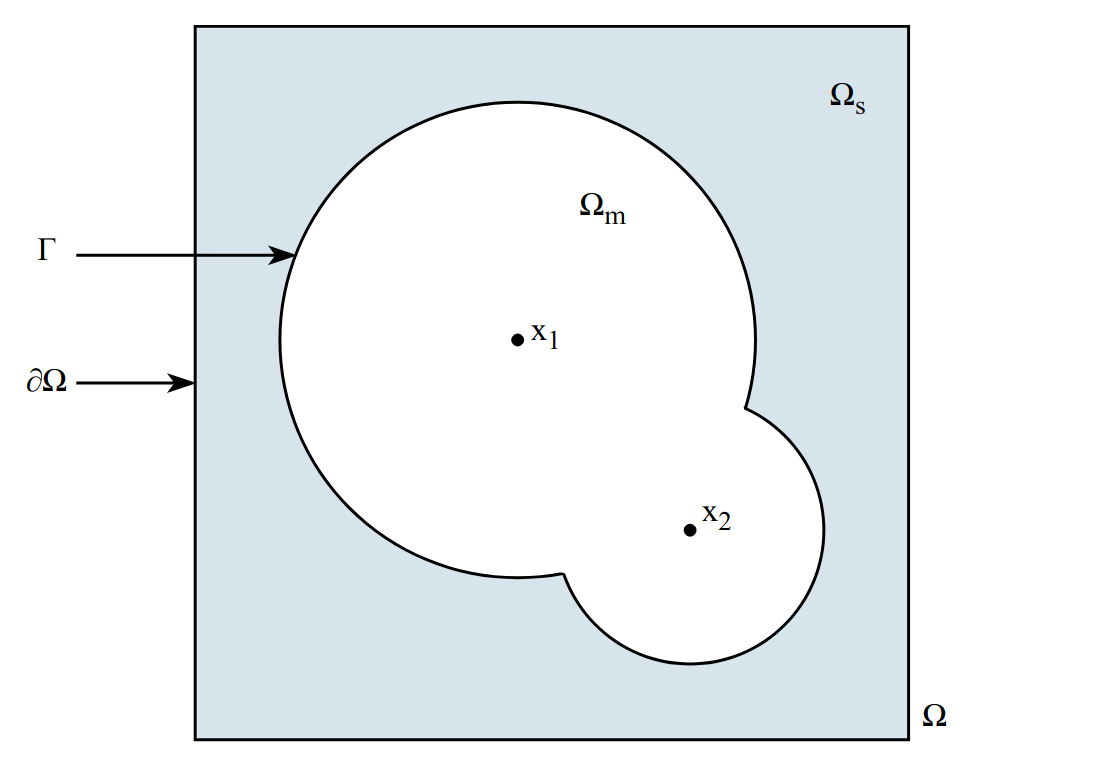
\includegraphics[width=0.65\textwidth]{Images/dominio.jpg}
    \caption{Schematic representation of the problem domain.}
\label{fig:domain}
\end{figure}

In order to introduce the mathematical statement of the PBE problem let us
start by defining the geometry of the domain where the problem is set.
To that end, consider the schematic 2D representation of Figure~\ref{fig:domain} 
and let the computational domain  $\Omega$ be defined as $\Omega \equiv 
\mathrm{Int}\left(\overline{\Omega}_m\bigcup\overline{\Omega}_s\right), \Omega 
\subset \mathbbm{R}^d$, where the interior of the molecule is denoted
by $\Omega_m$, and the solvent by $\Omega_s$. 

While solving the equation, both the solute and the solvent 
are treated as continuum media, each one characterized by its dielectric coefficient.

For a proper description of the problem physics, at least two different values for 
the coefficient are necessary. The difference between the two is due to the fact 
that the solvent is more easily polarized by an electric field, so that it is 
generally characterized by a higher dielectric  constant  $\varepsilon_s$, 
while the solute dielectric  constant $\varepsilon_m$ is about two orders 
of magnitude smaller.

Usually the relative electric permittivity is assumed to take the form
\begin{equation}
    \left\{
    \begin{aligned}
     & \varepsilon_r(x) = \varepsilon_s(x) & \mbox{in } \Omega_s \\ 
    & \varepsilon_r(x) = \varepsilon_m & \mbox{in } \Omega_m 
    \end{aligned}
    \right.
    \label{dielec}
\end{equation}

According to \eqref{dielec}, the relative electric permittivity is uniform inside
the solute, whereas it is a smooth function of the position $x$ in $\Omega_s$. 
This implies that  $\varepsilon_r$ is  discontinuous across the interior boundary $\Gamma = \partial \Omega_s \cap \partial \Omega_m$ which represents the \emph{molecular surface}.

The electrostatic potential is related to the \emph{fixed charge density}
$\rho^f$ and to the \emph{density of solution ions} $\rho^s$ by the Poisson equation
\begin{equation}
    \left\{
    \begin{aligned}
     & -\nabla \cdot \left(\varepsilon_0\ \varepsilon_r(x)\ 
    \nabla \varphi(x) \right)  =  \rho^s + \rho^f
     & \mbox{in } \Omega \\ 
    & \varphi(x) = g(x)  & \mbox{on } \partial \Omega,
    \end{aligned}
    \right.
    \label{eq:poisson}
\end{equation}
 where $\varphi$ is the unknown scalar electrostatic potential and $\varepsilon_0$ is the electric permittivity of vacuum.
 
The PBE is obtained by assuming that the density of charge in the solvent 
obey an equilibrium Boltzmann distribution, so that it can be expressed
as a function of the electrostatic potential.

In the most simple case (where only monovalent ions are assumed) such function
may be expressed as

\begin{equation}
 \rho^s = -2 e C^0 \sinh \Big(\frac{e\ \varphi}{k_B T}\Big),
 \label{rho_s}
\end{equation}
 where $k_B$ is the Boltzmann constant, $T$ is the absolute temperature and $e$ is the electron charge. The bulk concentration of monovalent species $C^0$, 
 is often expressed in terms of  the \emph{ionic strength} $I$ as
\begin{equation*}
    C^0 = 1000N_{AV}I,
\end{equation*}
where $N_{AV}$ is the Avogadro number and $I$ is expressed as a 
molar concentration.

Substituting~\eqref{rho_s} into~\eqref{eq:poisson} and assuming the fixed
charge density to be given by 
\begin{equation}
\rho^f = \sum_i q_i\ \delta(x-x_i),
    \label{eq:rhof}
\end{equation}
where the  points $x_i$ are the centers of the atoms composing the molecule, 
and the values $q_i$ their charges, we end up wit the semilinear PBE

\begin{equation}
    \left\{
    \begin{aligned}
     & -\nabla \cdot \left(\varepsilon_0\ \varepsilon_r(x)\ 
    \nabla \varphi(x) \right) + 2 e C^0 \sinh \Big(\frac{e\ \varphi}{k_B T}\Big)  =
    \sum_i q_i\ \delta(x-x_i)
     & \mbox{in } \Omega \\ 
    & \varphi(x) = g(x)  & \mbox{on } \partial \Omega.
    \end{aligned}
    \right.
    \label{eq:pbe_prob}
\end{equation}

The boundary condition $g(x)$ in \eqref{eq:pbe_prob} can be set in different
ways and we refer the interested reader to, {\it e.g.},~\cite{ROCCHIA20051109},
in what follows we will mostly assume, for sake of simplicity, that $g(x) = 0$.

If $\varphi (x)$ is not too large  w.r.t. $k_B T$, the semilinear PBE can be 
linearized by approximating the $\sinh$ term with a linear function, which leads 
to the following \emph{linearized} PBE
\begin{equation}
    \left\{
    \begin{aligned}
     & -\nabla \cdot \left(\varepsilon_0\ \varepsilon_r(x)\ 
    \nabla \varphi(x) \right) + 2 \left(\frac{e^2}{k_B T}\right) C^0 \varphi  =
    \sum_i q_i\ \delta(x-x_i)
     & \mbox{in } \Omega \\ 
    & \varphi(x) = g(x)  & \mbox{on } \partial \Omega.
    \end{aligned}
    \right.
    \label{eq:linpbe}
\end{equation}

The major problems to face while trying to solve \eqref{eq:linpbe} are the following:
\begin{enumerate}
    \item the very large scale algebraic systems of equations, due to the complex structure of the examined molecules, which require the adoption of HPC techniques for the solution of the problem;
    \item the discontinuity of the dielectric coefficient across the interface between the solvent and molecule;
    \item the presence of point sources, which can generate singularities in the problem solution and coefficients.
\end{enumerate}
In order to deal with all these aspects, we adopted some mathematical and numerical tools and approaches that will be described in detail in the following sections. 

\subsection{Scaling and Dimensionless Formulation}
\label{sec:dimensionless_form}

Before proceeding to solve either~\eqref{eq:pbe_prob} or~\eqref{eq:linpbe} it is useful 
common practice to perform a scaling procedure to transform them into their nondimensional 
counterpart. The purpose of such procedure is, on one hand, to scale the variables and coefficients
in the problem so that their numerical values are more amenable to numerical representation while,
on the other hand simplifying the notation by grouping several dimensional coefficients into
few dimensionless numbers.

To perform the scaling, we start by  expressing each physical quantity in \eqref{eq:poisson} 
as the product of a \emph{scaling factor} (with physical dimensions, identified in what follows 
by the  $\Bar{\cdot}$ symbol) and a \emph{dimensionless} 
variable denoted by the $\hat{\cdot}$ symbol, {\it i.e.}:
\begin{equation}
\begin{aligned}
    \label{scalingfactors}
     \varphi & := \Bar{\varphi}\hat{\varphi} \\
    x & := \Bar{x}\hat{x} \\
     \rho^s & := \Bar{\rho}\hat{\rho}^s \\
    \rho^f & := \Bar{\rho}\hat{\rho}^f.
\end{aligned}
\end{equation}

Table~\ref{table:scalingfacts} shows the most common choices for the scaling factors, which
are used in the implementation of {\tt easy\_pbe}.

Using the notation in~\eqref{scalingfactors}, dividing both sides of~\eqref{eq:poisson} by $\Bar{\rho}$, and assuming $\Bar{\varphi} = \dfrac{k_B T}{e}$ (which is the most common choice
for the scaling factor for electrostatic potential) leads to 

\begin{equation}
    -\frac{\varepsilon_0\ \Bar{\varphi}}{\Bar{x}^2 \Bar{\rho}}\ 
    \hat{\nabla} \cdot \left( \varepsilon_r\ 
    \hat{\nabla} \hat{\varphi} 
    \right) -  \hat{\rho}^s
        =  \hat{\rho}^f,
\end{equation}
which, upon defining 
$$ \hat{\varepsilon}_0 := \frac{1}{\Bar{\rho}\ \Bar{x}^2}\ \varepsilon_0\ \Bar{\varphi} $$
becomes
\begin{equation}
- \hat{\nabla} \cdot \left( \hat{\varepsilon}_0\
 \varepsilon_r\ 
    \hat{\nabla} \hat{\varphi} 
    \right) - \hat{\rho}^s
    = \hat{\rho}^f.
\end{equation}

Introducing the \emph{scaled ionic force coefficient} $\hat{I} := \frac{2eC^0}{\Bar{\rho}}$, 
letting $ \hat{\varepsilon}_0\ \varepsilon_r \kappa^2 := \hat{I}$
and the nondimensional atomic charges $\hat{q}_i = \frac{q_i}{\Bar{x}^3 \Bar{\rho}}$
the semilinear version of the PBE can now be written as
$$
- \hat{\nabla} \cdot \left( \hat{\varepsilon}_0\
 \varepsilon_r\ 
    \hat{\nabla} \hat{\varphi} 
    \right) +  \hat{\varepsilon}_0\ \varepsilon_r \kappa^2 \sinh\left(\hat{\varphi}\right)
    = \displaystyle \sum_i \hat{q}_i\ \delta (\hat{x} - \hat{x}_i)
$$
while the linearized, nondimensional form becomes
\begin{equation}
    - \hat{\nabla} \cdot \left( \hat{\varepsilon}_0\
 \varepsilon_r\ 
    \hat{\nabla} \hat{\varphi} 
    \right) +  \hat{\varepsilon}_0\ \varepsilon_r \kappa^2 \hat{\varphi}
    = \displaystyle \sum_i \hat{q}_i\ \delta (\hat{x} - \hat{x}_i).
    \label{eq:adimensionalpbe}
\end{equation}

\begin{table*}
\centering 
    \begin{tabular}{| c | c |}
    \hline
     \rowcolor{bluePoli!40}
      \textbf{Scaling Factor} & \textbf{Value}  \T\B \\
    \hline 
    $\Bar{\varphi}$ & $k_BT / e$ 
    \T\B\\
    $\Bar{x}$  & 1 \AA 
    \T\B\\
    $\Bar{\rho}$  & $e / (4 \pi \Bar{x}^3)$
    \B\\
    \hline
    \end{tabular}
    \\[10pt]
    \caption{Choice of scaling factors.}
    \label{table:scalingfacts}
\end{table*}

For the sake of easing the notation, we will henceforth drop the $\hat{\cdot}$ symbol
and consider the PBE to be expressed in nondimensional form.

\subsection{Treatment of Point Sources}
\label{sec:point_sources}
As anticipated in the previous section, the presence of point sources induces 
singularities in the analytical solution of the PBE that are one of the main
issues in the numerical solution of the problem.

Two main approaches can be used to deal with such issue, namely ({\it i}) adopting
a \emph{regularized} reformulation of the problem~\eqref{eq:adimensionalpbe} that removes
the point sources by accounting for their presence by means of a surface charge density 
either on $\Gamma$ or on $\partial \Omega$; or ({\it ii}) adopting a \emph{smoothed} representation of the atomic charges, {\it i.e.} representing them as finite charge density
distribution functions with a small and compact, yet finite, support.

The first approach can be pursued in different ways that all exploit the availability of explicit expressions for the Green functions for the differential operator in~\eqref{eq:adimensionalpbe}, a review of a variety of such ways is given in~\cite{ref16}, here we only give and example of such approach in Section~\ref{sec:regularization}, which is not currently implemented in {\tt easy\_pbe}.

The approach ({\it ii}) can also be implemented in different ways, 
but the most natural one in the framework of {\tt easy\_pbe} relies on
expressing the atomic charges as linear combinations of Finite Element shape
functions and is described in Section~\ref{sec:chargedeposition} below.

\subsubsection{Representing Atomic Charges via FEM Shape Functions}
\label{sec:chargedeposition}

As {\tt easy\_pbe} adopts a Finite Element discretization for solving the
PBE, the most natural way of defining a continuous function with finite
support consists of representing it as a linear combination of Finite Element
shape functions.

In particular, as {\tt easy\_pbe} uses continuous first-order Lagrangian Finite 
Elements, the degrees of freedom of each shape function are collocated at one
of the cell vertices, therefore the natural choice consists of defining 
the $i$--th smoothed atomic charge density function $\rho_i(x)$ as

$$
\rho_i(x) := \sum_k N_k(x) q_{ik},
$$
where $ N_k(x) $ denotes the shape function relative to the $k$--th mesh vertex
and $q_{ik}$ are the values of $\rho_i$ at that vertex.

The main constraint that the nodal values $q_{ik}$ must obey is that of preserving
the total amount of charge, {\it i.e.}
$$
\int_\Omega \rho_i(x)\ \mathrm{d}\omega = \sum_k q_{ik}  \int_\Omega N_k(x) \ \mathrm{d}\omega = q_i.
$$
A simple choice that satisfies this latter constraint is setting
$$
q_{ik} := q_i \dfrac{N_k(x_i)}{\int_\Omega N_k(x) \ \mathrm{d}\omega }.
$$
Indeed, from this definition it follows that
$$
\int_\Omega \rho_i(x)\ \mathrm{d}\omega = q_i \displaystyle \sum_k
N_k(x_i) \dfrac{\int_\Omega N_k(x) \ \mathrm{d}\omega}{\int_\Omega N_k(x) \ \mathrm{d}\omega} = q_i \displaystyle \sum_k
N_k(x_i) = q_i,
$$
where the last inequality discends from the fact that the basis functions
enjoy a \emph{partition of unity} property. 

Notice that, for first-order continuous Finite Elements, if the atom center 
$x_i$ lies in a cell $ \tau $, only the basis functions that are collocated
at the vertices of $\tau$ are non vanishing at $x_i$ therefore the weights
$q_{ik}$ are non vanishing only for a small set of values of $k$\footnote{For
a tensor-product hexahedral cartesian mesh, this would be exactly 8 values of $k$,
but given that we use a refined mesh with hanging nodes the number of non vanishing coefficients depend on the mesh refinement.}.
 
 \subsubsection{Example of Regularized Formulation Without Point Charges}
 \label{sec:regularization}
The point charges can be eliminated from the problem introducing one of the so-called \emph{regularization techniques}. We consider one example of these techniques which transfers the effect of the point charges to the boundary conditions and to the interface condition on $\Gamma$.  
Let's start considering the nondimensional semi-linear boundary value problem with homogeneous Dirichlet boundary conditions on $\partial\Omega$, namely

\begin{equation}
    \left\{
    \begin{aligned}
     - & \nabla \cdot \left( \varepsilon_0 \varepsilon_r(x)\ 
    \nabla \varphi(x) \right)  =\ - \varepsilon_0 \varepsilon_r (x) \kappa^2 \varphi (x)
    + \sum_i q_i\ \delta(x-x_i) & \mbox{in } \Omega \\ 
    & \varphi = 0 & \mbox{on } \partial \Omega 
    \end{aligned}
    \right.
    \label{eq:pbe_prob_dir}
\end{equation}
\\
We decompose $\varphi (x)$ as $\varphi (x) = \varphi_s (x) + \varphi_m (x)$, where $\varphi_m (x)$ is the contribution
to the electrostatic potential due only to point sources, while $\varphi_s (x)$ accounts for the correction
due to the surface polarization charge related to the discontinuity in the permittivity. If the dielectric permittivity were independent from position $x$, the scalar electrostatic potential due to the i-th point charge and $\varphi_m (x)$ would be respectively

\begin{align*}
    \varphi_i (x) & = \frac{q_i}{4 \pi \varepsilon_0 \varepsilon_m\ |x-x_i|} \\
    \varphi_m & (x) = \sum_i \varphi_i (x)
\end{align*}

Then the potential correction $\varphi_s (x)$ is given by the difference between the exact electrostatic potential and the one only due to point source charges
\begin{equation}
    \varphi_s (x) = \varphi (x) - \varphi_m (x).
    \label{correct_pot}
\end{equation}

Since no point sources are present in $\Omega_s$, the equation in the solvent domain becomes

\begin{equation}
    -\nabla \cdot (\varepsilon_0 \varepsilon_m\ \nabla \varphi_m) (x) = - \varepsilon_0 \varepsilon_m\ \Delta \varphi_m = 0 \mbox{, in } \Omega_s
    \label{point_source_pot_in_solvent}
\end{equation}

We start from the equation in (\ref{eq:pbe_prob_dir}) restricted to the solvent domain $\Omega_s$. Exploiting both the observation made in (\ref{point_source_pot_in_solvent}) and the definition of the potential correction (\ref{correct_pot}), we obtain
\begin{equation*}
\centering
\begin{aligned}
        - \nabla \cdot (\varepsilon_0 \varepsilon_s (x) \nabla \varphi_s ) & = - \nabla \cdot (\varepsilon_0 \varepsilon_s (x) \nabla (\varphi - \varphi_m) ) \\
        & = - \nabla \cdot (\varepsilon_0 \varepsilon_s (x) \nabla \varphi) + \varepsilon_0 \varepsilon_s \Delta \varphi_m + (\varepsilon_0 \nabla \varepsilon_s ) \cdot (\nabla \varphi_m) \\
        & = - \varepsilon_0 \varepsilon_s \kappa^2 (\varphi_s + \varphi_m) + (\varepsilon_0 \nabla \varepsilon_s ) \cdot (\nabla \varphi_m).
\end{aligned}
\end{equation*}

While at the interface $\Gamma$
\begin{equation*}
    0 = [[-\varepsilon_r \nabla \varphi \cdot n]]_{\Gamma} =  [[- \varepsilon_r \nabla \varphi_s \cdot n]]_{\Gamma} - [[ \varepsilon_r]]_{\Gamma} (\nabla \varphi_m)|_{\Gamma} \cdot n,
\end{equation*} 
where $[[\cdot]]_{\Gamma}$ represents the jump of quantity between brackets across the interface. \\\\
Finally, on the domain boundary $\partial \Omega$, substituting the definition of the potential correction (\ref{correct_pot}), inside the Dirichlet boundary conditions of problem (\ref{eq:pbe_prob_dir}) we obtain
\begin{equation*}
    \varphi(x)|_{\partial\Omega} = (\varphi_s (x) + \varphi_m (x))|_{\partial\Omega} = 0.
\end{equation*}

Therefore, reformulating the problem  (\ref{eq:pbe_prob_dir}) w.r.t. $\varphi_s (x)$, it becomes

\begin{subequations}
    \label{eq:pbe_no_point_sources}
    \begin{align*}[left=\empheqlbrace]
    & - \nabla\cdot ( \varepsilon_0 \varepsilon_s (x)\ \nabla \varphi_s) = (\varepsilon_0 \nabla \varepsilon_s) \cdot \sum_i \nabla \Big( \frac{q_i}{4 \pi \varepsilon_0 \varepsilon_m |x - x_i|} \Big) - \varepsilon_0 \varepsilon_s \kappa^2 \Big(\varphi_s +  \sum_i \frac{q_i}{4 \pi \varepsilon_0 \varepsilon_m |x - x_i |} \Big) & \mbox{ in } \Omega_s \\
    & - \Delta \varphi_s = 0 & \mbox{ in } \Omega_m  \\
    & [[- \varepsilon_r \nabla \varphi_s \cdot n]]_{\Gamma} = [[ \varepsilon_r]]_{\Gamma} \nabla \varphi_m \cdot n & \mbox{ on } \Gamma  \\
    & \varphi_s (x) = \sum_i \frac{q_i}{4 \pi \varepsilon_0 \varepsilon_m |x - x_i|} & \mbox{ on } \partial \Omega 
    \end{align*}
\end{subequations}
 which has no point charges. Notice that third relation of the above system is expressed in $[C/m^2]$ SI units, so that it can be interpreted as a surface charge distribution. The main advantage of this regularization technique is to avoid the need of using small mesh sizes in $\Omega_m$, but only at the molecular surface.

\section{Geometric Representation of the Molecular Surface}
\label{sec:molecular_surf}

The representation of the molecular surface $\Gamma$ is a focal point of research 
in numerical methods for implicit solvent continuum models of biomolecular systems.

Given the positions $x_i,\, i = 1 \ldots n_a $ of the atomic centers and the
atomic radii $r_i$, one has to define the 2D manifold $\Gamma$, and this can
of course be accomplished in many different ways, the choice among which is
guided by several characteristics of the generated surface.

The main requirement is, of course, the accuracy of the electrostatic computation
results, which is usually measured by comparison to results of solvent explicit
computations. In addition to this, though, other properties are to be taken into 
account such as, for example, the differentiability of the surface w.r.t. to the 
atomic positions and radii and the continuity of the molecular surface area w.r.t.
the atom positions.

The arguably most simple approach to the surface definition is the so called 
\emph{Van der Waals} approach, according to which the molecular domain
is defined as the union of the spherical regions centered at $x_i$ and 
with radius $r_i$.

In~\cite{ref8}, a comparison of three approaches is given, namely
\begin{enumerate}
    \item \emph{Blobby surface},
    \item \emph{Skin surface},
    \item \emph{Solvent Excluded Surface} (SES), a.k.a. Connolly surface.
\end{enumerate}

These  three options are all implemented in {\tt easy\_pbe}, the first one via a
native implementation, the latter two via an interface to the geometrical library
{\tt NanoShaper}~\cite{RDCNS} and are therefore described in detail below.

%The first one is based on an implicit level-set representation while the latter two rely on alpha-shapes, a parametrized generalization of the convex hull concept. The alpha-shape is the geometric dual of the space-filling model of the molecule, with parameter $\alpha$ which corresponds to a specific degree of detail in the description of the shape. \\
%The efficient construction of the surface and the evaluation of its interior and exterior regions is a significant aspect when considering the overall simulation complexity, for this reason much effort during the development of the thesis has been put in constructing an effective interface with the NanoShaper
%library \cite{ref8} to deal with this task. 

\subsection{Blobby Surface}
\label{sec:blobby}
Blobby surface, proposed in \cite{blobby1, blobby2}, is an implicit surface whose definition is based on Gaussian atom center idea. Any implicit surface can be visualized using a ray-tracing technique which consists in finding  all the points where an intersection with the surface occurs by tracing rays along a prescribed direction. \\ 
Its mathematical definition is quite simple and intuitive: it is the level set $S$, see Figure \ref{fig:blobby}, of a particular function $G(x)$, namely

\begin{equation}
    S := \{ x \in \mathbbm{R}^3 : G(x) = 1  \},  
    \: \: \: \: \: \: \: \: \: \: \: 
    G(x) = \sum_{i=1}^{n_a} \exp\Big({B \Big( \frac{|| x - x_i ||^2}{r_i^2} - 1 \Big) }\Big),
\label{blobby}
\end{equation}

where $x$ represents a point over the surface, while $B$ is the \emph{blobbyness}, a parameter that controls the surface roughness and that has to be tuned. Then there are three quantities that describe the chosen molecule: $n_a$, the number of atoms inside the molecule, $r_i$ which is the radius of the i-th atom and $x_i$, the vector of coordinates of the i-th atom center. 

\begin{figure}[H]
    \centering
    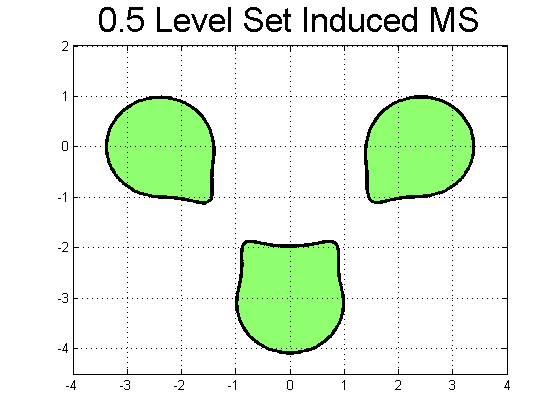
\includegraphics[width=0.45\textwidth]{Images/Blobby.jpg}
    \caption{0.5 level-set, Blobby surface \cite{ref8}.}
\label{fig:blobby}
\end{figure}

Even if the usage of this kind of surface is fascinating because, due to its simple definition, it is easy to implement, also in parallel, it is not so easy to define a projection method for a point over the surface.  Indeed, contrary to the Skin and SES surfaces, it cannot be partitioned in analytical patches. Another thing to point out is that while on one side it is appreciated for its smoothness which guaranties continuity and differentiability without any self-intersection nor singularities, on the other side it is not superior to the Connolly surface for the solution of electrostatic problems. Moreover, the choice of the \emph{blobbyness}, which is a key parameter for the calculus of the energy estimates of the molecules, can create some problems. All these drawbacks lead to prefer Skin and SES surface for more accurate results. 

\subsection{Skin Surface}
\label{sec:skin}
The Skin surfaces, as the Blobby, is an implicit surface appreciated for its smoothness and because it is expected to provide a surface area continuous with respect to atom positions and radii.
Its definition was proposed in \cite{MixedCell}, and it is more complex from a mathematical point of view.
It can be constructed starting from a set of weighted points $S$ and a shrink factor $s$ $\in$ (0, 1]. The latter is the characterizing parameter for the Skin surface that has to be set, similarly to the \emph{blobbyness} $B$ in the Blobby case.  The set $S$ and the weights of the points $w_i$ can be defined as follows:

\begin{equation}
    \begin{aligned}
        S = \big{\{} p_i = ( x_i, w_i ),
        \: \: &x_i \in \mathbbm{R}^3, 
        \: \: i = 1,..., n_a \big{\}}  \\
        w_i &= \frac{r_i^2}{s}
    \end{aligned}
\label{skin}
\end{equation}
where $n_a$ is the number of atoms inside the considered molecule and $r_i$ and $x_i$ are respectively the radius and the center of the i-th atom. \\
For defining precisely the Skin surface, the concept of \textit{mixed complex} has to be introduced, since starting from it the surface equations can be derived. 
The \textit{mixed complex} is composed of \textit{mixed cells} $\mu_X^s$ which are solids that can be computed through the Minkowsky sum "$\oplus$", as reported in (\ref{mixed_cells}), exploiting either the Voronoi diagram or Delaunay tetrahedrization.

\begin{equation}
    \label{mixed_cells}
    \mu_X^s = \{ s \cdot \nu_X \oplus (1 - s) \cdot \delta_X \} 
\end{equation}
In this definition, $X$ is a subset of a finite set of spheres in $\mathbbm{R}^3$ and $\nu_X$ is a non empty Voronoi cell with corresponding Delaunay simplex $\delta_X$ \cite{MixedCell}. After the \textit{mixed cells} are calculated, a ray-tracing software can be used in order to define the inside and outside of the surface. A schematic representation of both the \textit{mixed complex} and Skin surface of a simple molecule where 8 equal atoms are put on the vertices of a cube can be seen in Figure \ref{fig:skin}. 

\begin{figure}[H]
    \centering
    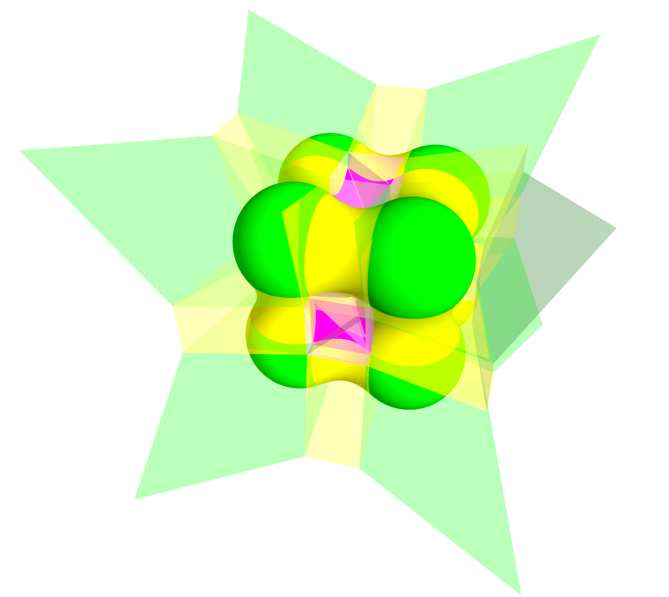
\includegraphics[width=0.45\textwidth]{Images/skin.png}
    \caption{Skin Surface and mixed complex (transparent). Surfaces corresponding to $\mu_{3,0}^s$, $\mu_{2,1}^s$, $\mu_{1,2}^s$ \emph{mixed complex} are represented in green, yellow and magenta, respectively \cite{ref8}.}
\label{fig:skin}
\end{figure}

The existence of such fast algorithms as Voronoi diagram or Delaunay tetrahedrization for the construction of the Skin surface constitutes an advantage with respect to other kind of surfaces. In addition, also the presence of pathological configurations which can create normal discontinuities are extremely limited. In any case, the computational costs are higher than the Connolly ones and, moreover, Skin surface can create unphysical high dielectric cavities, regions that can affect the energy estimate of the system.

\subsection{Connolly Surface}
\label{sec:connolly}
The SES is one of the most commonly adopted molecular surfaces in Computational Biological Chemistry for the visualization of the surface area. This kind of molecular surface was suggested by Lee and Richards in \cite{LeeRich} but it is commonly known as Connolly surface, so called because of the famous algorithm computation proposed by Connolly. \\
For defining the Connolly surface, we start from a simpler definition of molecular surface, in which it is defined as the contact surface between the Van der Waals envelope of the solute molecule and the probe solvent molecule. The Van der Waals surface is the enclosing surface obtained by the superposition of hard spheres which represent the atoms present inside the examined solute molecule. The union of all the hard spheres forms the Van der Waals volume and each of those spheres has radius equal to the Van der Waals radius, that is calculated as a distance between atoms in crystals and indicates the largest distance at which an atom repels its neighbors. 
On the other hand, considering the solvent molecules, Solvent Accessible Surfaces (SAS) are adopted. This kind of surface can be described as the locus of the centers of a spherical probe that rolls over the molecular system. This kind of surface coincides geometrically with the Van der Waals surface, where each radius of the above described hard spheres is increased by the probe radius size. 
Starting from SAS, further developments lead to the Solvent Excluded Surface (SES), which separates the finite volume accessible to a finite size solvent probe from the inaccessible one. Indeed, also SES surface is computed by rolling the probe sphere over the van der Waals surface of the molecule, but in this case the surface is determined by the surface of the probe, instead of its center. Figure \ref{fig:SESvsSAS} shows schematically the difference between SAS, SES anche the Van der Waals surface, while Figure \ref{fig:connolly} represents a simple example of Connolly surface in 3D. 

\begin{figure}[H]
    \centering
    \subfloat[Schematic representation of the difference between SES, SAS and Van der Waals surface, with an example of probe.\label{fig:SESvsSAS}]{
        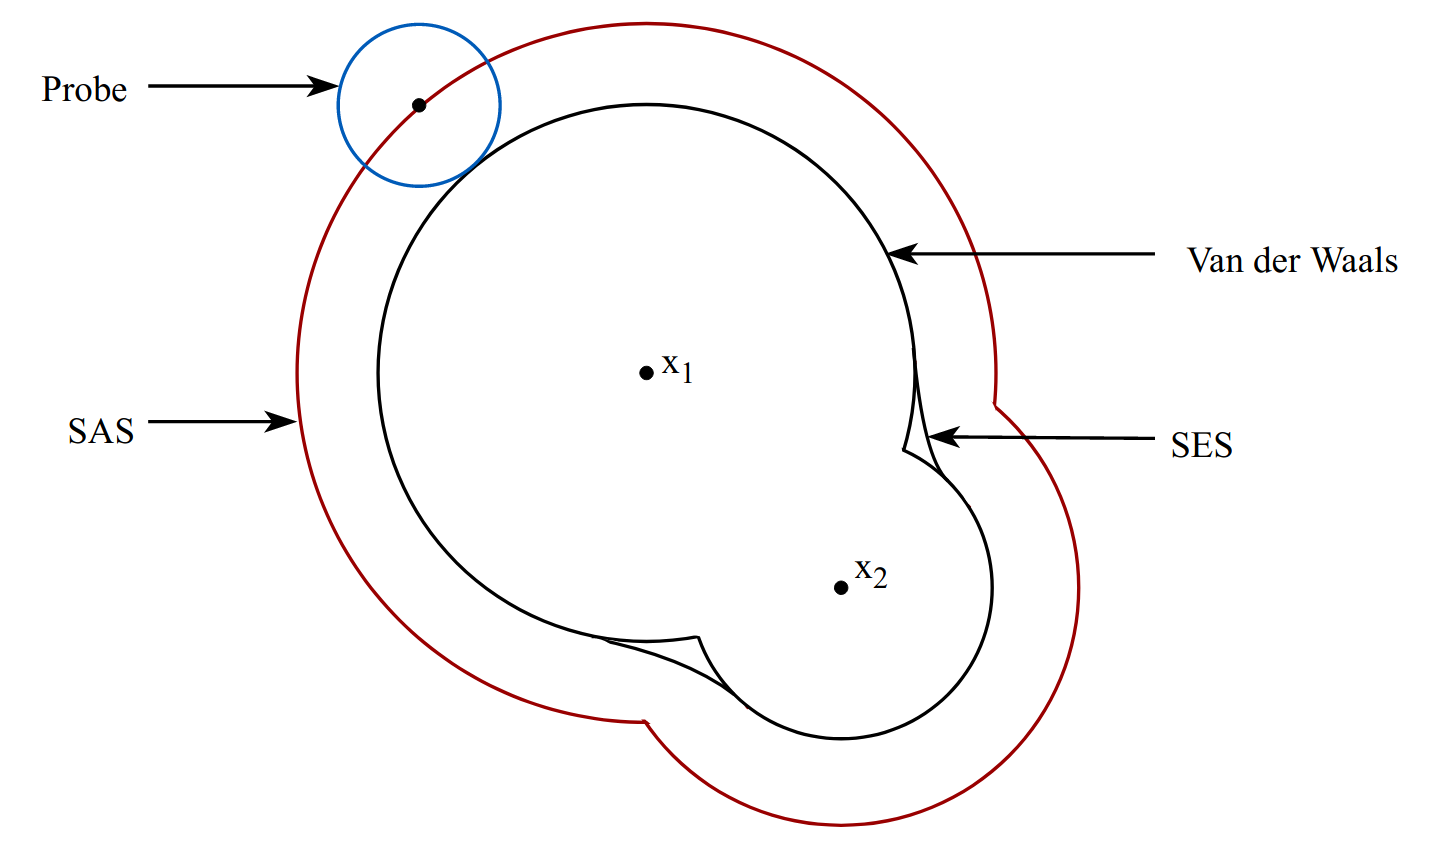
\includegraphics[scale=0.16]{Images/SES_SAS_W_diag.png}
    }
    \quad
    \subfloat[Connolly surface \cite{ref8}.\label{fig:connolly}]{
        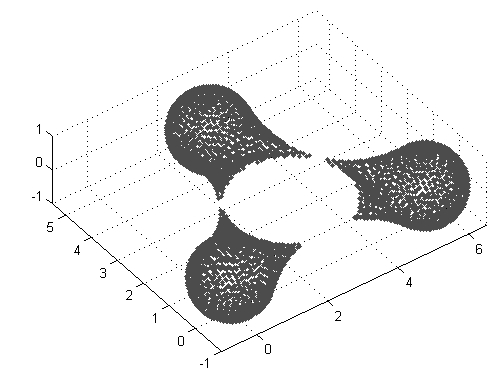
\includegraphics[scale=0.4]{Images/connolly.jpg}
    }
    \caption[]{}
    \label{fig:SES}
\end{figure}

The Connolly surface is appreciated because it is conceptually simple, but on the other hand it can present some singularities and a discontinuous dependence of the surface area on the position of atom centers. 

\section{Oct-tree grids}
\label{sec:octree}
The very large size and complex structure of the molecules being studied leads to very large scale algebraic systems of equations which demand for state-of-the-art HPC solver technology. The novelty of this work w.r.t. the already existing PBE solvers consists in solving the linearized Poisson--Boltzmann equation with Finite Element method on Oct-tree, which are hierarchically refined, non conforming, cartesian grids. Indeed, typically the other solvers calculate the electrostatic potential adopting either tensor product cartesian grids with simple numerical methods, which is characterized by high memory efficiency, but it is not so accurate, or adaptive, simplicial, conforming meshes with Finite Differences method, less efficient and more accurate. The choice of Oct-tree grids gives our solver benefits in terms of efficient parallel partitioning, refinement, coarsening and balancing, while FE is more flexible for local mesh refinement. \\
The structure of an Oct-tree grid can be easily represented as a tree (Figure \ref{fig:octree_tree}), as the name suggests, where each octant ({\it i.e.} each element of the mesh, see Figure \ref{fig:octree_octant}) is a either a leaf or has 8 children. Indeed, the mesh is generated starting from a 3D cube and then iteratively refining or coarsening the elements in a non conforming way. 

\begin{figure}[H]
    \centering
    \subfloat[Example of a simple Oct-tree mesh.\label{fig:octree_octant}]{
        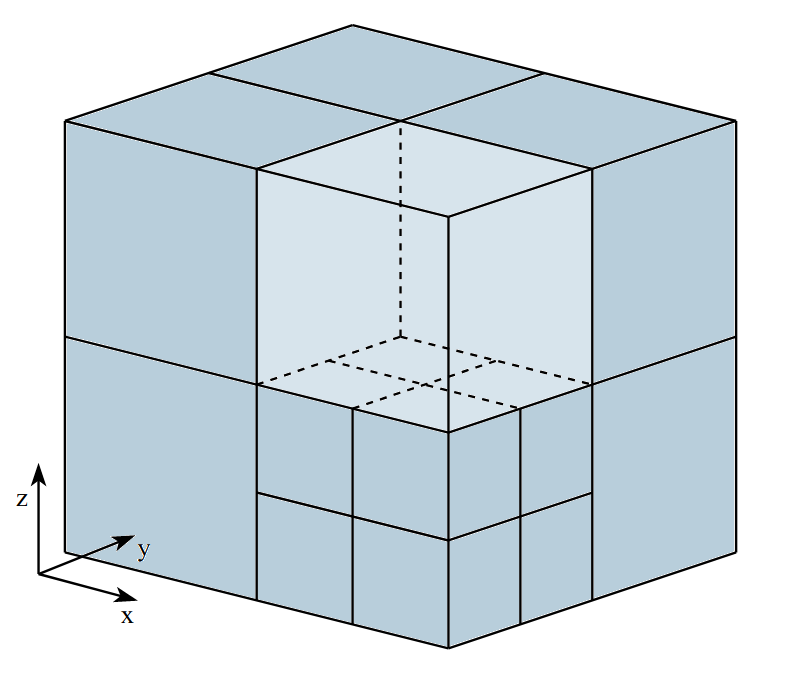
\includegraphics[scale=0.4]{Images/octreegrid.png}
    }
    \quad
    \subfloat[Tree associated to the Oct-tree grid.\label{fig:octree_tree}]{
        \includegraphics[scale=0.26]{Images/tree.png}
    }
    \caption[]{}
    \label{fig:octree}
\end{figure}

More in detail, the starting 3D cubic domain is initially uniformely refined in a rough manner in order to obtain a first solution, that will be used as a starting point for the following refine-coarsen iterations. Then, the idea is to divide a mesh element into 8 smaller cubes when it contains either an atom charge or part of the molecular surface, and coarsen the grid otherwise. 

The initial level of refinement is indicated as level 0, then if one element belonging to level 0 is refined N times, each of the resulting subelements belongs to level N. Each cubic element of the mesh is characterized by the same numbering of faces, edges and nodes, which is the one reported in Figure \ref{fig:quadtree}. All these enumerations, jointly with the quadrant indexing too, follow the z-ordering. \\

\begin{figure}[H]
    \centering
    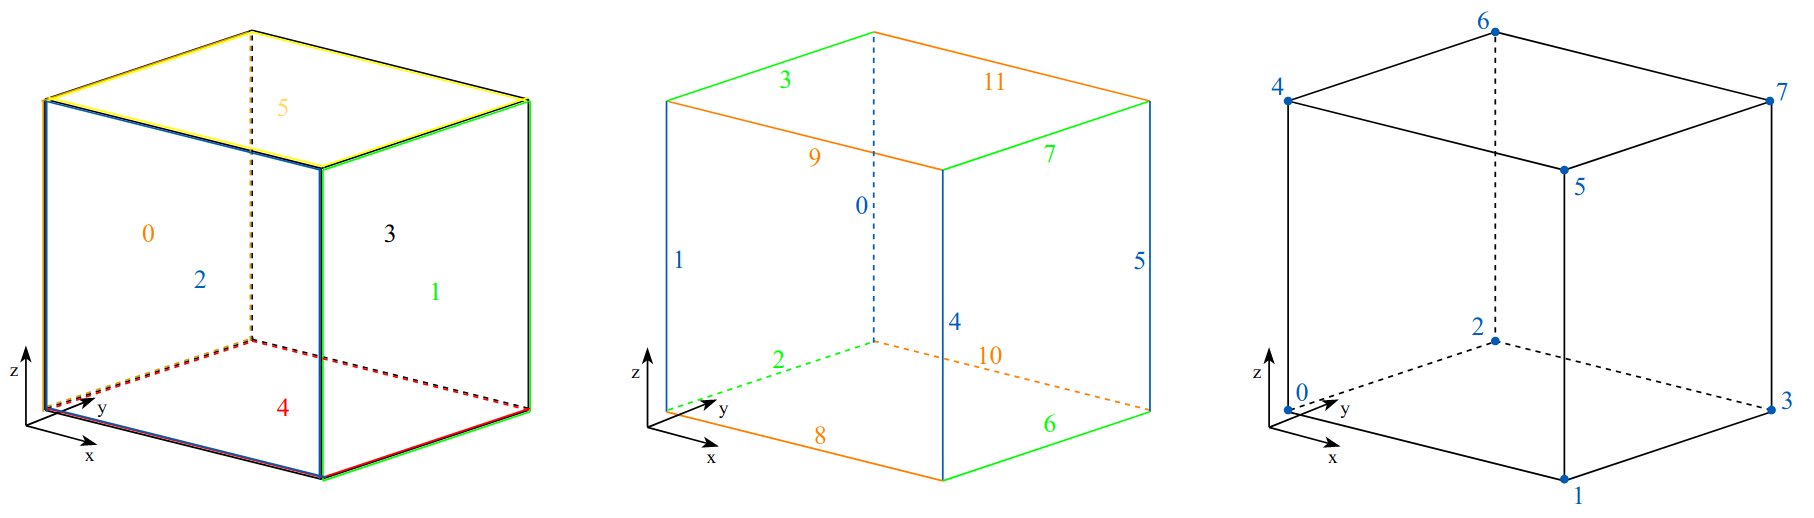
\includegraphics[width=0.9\textwidth]{Images/enum.jpg}
    \caption{From left to rigth: numbering of faces, edges, nodes of each quadrant.}
    \label{fig:quadtree}
\end{figure}

The quadrant numbering is particularly important in parallel applications because it produces a smart subdivision of the mesh octants among the involved processors. This operation takes the name of parallel partitioning and is performed according to a given number of elements per processor or according to some prescribed
weights associated to those elements. To better understand in which way this is done, a simple example of the refinement process of a 2D Quad-tree mesh is reported below in Figure \ref{fig:quadtree2}. The initial square domain is split into four elements, all belonging to level 1 (Figure \ref{fig:refin1}). Then, only the element indicated with number 1 is refined and all the squares are renumbered as shown in Figure \ref{fig:refin2}. In the third step element 3 is divided into four subelements so that the enumeration changes again. The correlation between the quadrant numbering and the corresponding tree is pointed out in Figure \ref{fig:refin3}, where the Morton S-shaped space filling curve is reported. The nodes are subdivided among the processors following this curve, so that nodes belonging to the same processors are also neighbors in the mesh. This is useful in order to limit communications between processors.

\begin{figure}[H]
    \centering
    \subfloat[First refinement step.\label{fig:refin1}]{
        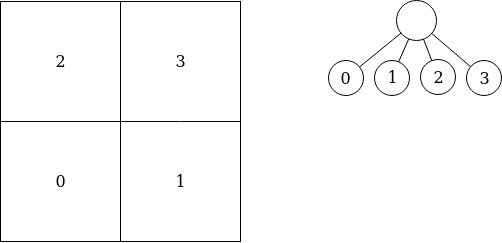
\includegraphics[scale=0.5]{Images/Refinement1.jpg}
    }
    \quad
    \subfloat[Second refinement step.\label{fig:refin2}]{
        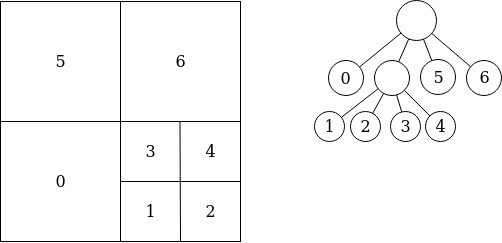
\includegraphics[scale=0.5]{Images/Refinement2.jpg}
    }
    \quad
    \subfloat[Third refinement step with Morton S-shaped space filling curve.\label{fig:refin3}]{
        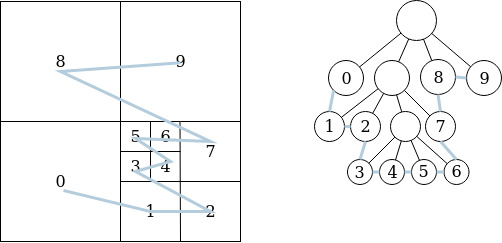
\includegraphics[scale=0.5]{Images/Refinement4.jpg}
    }
    \caption[]{Quad-tree mesh refinement example.}
    \label{fig:quadtree2}
\end{figure}

The resulting mesh is a non conforming mesh, in which at most 2:1 edge size relations between neighboring octant is ensured, that is the so-called balancing. This is done in order to properly deal with the hanging nodes. These kind of nodes are, in 2D case, nodes belonging to an edge which is refined for two elements, but not for the neighboring one, like for example two red marked nodes in Figure \ref{fig:hanging}. In the Oct-tree cases these nodes can be generated both on faces and on edges. Their main characteristic is that they present a local numbering, but no global numbering. In order to be identified, they are related to the global numbering of their non-hanging parents, \emph{i.e.} the nodes belonging to the same edge or face (the latter only in the 3D context) where the hanging node is present. Since hanging nodes are not present inside the set of the degrees of freedom, they have to be taken into account in a different way. 

\begin{figure}[H]
    \centering
    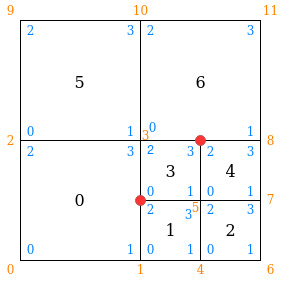
\includegraphics[width=0.3\textwidth]{Images/hanging.jpg}
    \caption{Example of hanging nodes, marked with red spots. Black numbers refer to quadrant numbering, blue to node local indices, orange to node global indices.}
    \label{fig:hanging}
\end{figure}

\section{Implementation strategy}
\label{sec:implementation}
During this thesis we have developed a parallel solver on adaptive meshes for the solution of the linearized PBE. The implemented code can be found inside this repository: \url{https://github.com/carlodefalco/easy_pbe}. \\
The user reference with the instructions on how to compile and use the code and for the output visualization can be found in Appendix \ref{App_A}. \\\\
To achieve our goals, the \texttt{bim++} library which provides at the same time a high-level access to meshes with a series of functions for the solution to PDEs in the FE method context and also a \texttt{c++} interface to \texttt{p4est} library, was adopted. Through \texttt{p4est} library it was possible to handle the Oct-tree grids and perform the hierarchical mesh refinement over the octants that compose the 3D domain, while the efficient construction of the molecular surface and the evaluation of its interior and exterior points, rely on \texttt{NanoShaper}. The latter is able to find some surface characteristics such as the volume of the molecule, the surface area and cavities (regions present inside proteins, big enough to contain one or more water molecules) through a ray-casting technique. It is possible to construct both SES and Skin surfaces, while the Blobby surface is not available for the \texttt{NanoShaper API}. For this reason this kind of surface was directly implemented inside the code using its definition (\ref{blobby}). 

\subsection{Code Description}
The main function of the code is the \texttt{poisson\_boltzmann.cpp} file, in which the functions and methods necessary for the computation of the electrostatic potential are called. The algorithm is composed of six steps, described in the subsections below.
\subsubsection{Data Input}
The first step consists in reading from the two input files selected by the user: the \texttt{options.pot} file, with the simulation parameters, and a .pqr file, containing the 3D molecular structure. The atom characteristic extracted from such file are stored in vector of \texttt{NS::Atom} class objects. The \texttt{Atom} class is defined in the \texttt{NanoShaper} library as reported below, where the member functions have been dropped for brevity. 
\begin{code}
class Atom: public Point
{
public:
	double radius;
	double radius2;
	double charge;
	int dielectric;
	AtomInfo ai;
	
	// *member functions*
};
\end{code}

\subsubsection{Surface Creation}
For the surface creation a query to \texttt{NanoShaper API} was introduced. This is done only by rank zero at the line
\begin{code}
ray_cache.init_analytical_surf (pb.atoms, pb.surf_type, pb.surf_param,    
                                     pb.stern_layer, pb.num_threads);
\end{code}
where the analytical surface is created starting from the atom characteristics, passed to \texttt{NanoShaper} through \texttt{pb.atoms}, that is the previously cited \texttt{std::vector<NS::Atom>}. \\
Once the analytical surface is created, the geometric surface can be defined by tracing the rays which start from one domain boundary face and arrive to the other. Through this technique, \texttt{NanoShaper} is able to stabilize where the molecular surface intersections occurs. This operation is performed in the following step.

\subsubsection{Mesh Creation and Refinement}
The Oct-tree grid is created and initialized accordingly to the user requests, then the refinement and coarsening operations can be performed. In
particular, at each iteration a loop over the octants of the mesh is done. The current cell is refined either if it contains at least one non hanging node inside the molecule and at least one in the solvent, which means the molecular surface is contained in the current element, or when it contains a point charge. During the coarsening iterations the
opposite idea is carried out: the mesh can be coarse where neither the point charges nor molecular surface are present and the 2:1 edge size relation between neighboring
octants is still respected. \\
In order to establish if a point is either inside or outside the molecule, we exploits the information about the intersection given by \texttt{NanoShapers} and assign to that point value 1 when it is inside the molecule, 0 if it is outside, -1 if unknown. The latter is returned only by the non-zero processors when the ray to which the point belongs is not present inside their \texttt{ray\_cache\_t} object. The design of the \texttt{ray\_cache\_t} class is explained in detail in the next paragraph. 

\subsubsection{Ray Caching}
\texttt{NanoShaper} can be executed either in serial or using multiple threads, while our solver parallelization rely on MPI which is based, instead, on multi-core processing. This difference leads us to implement a Master--Slave program, where the \texttt{NanoShaper} functions are explicitly called only by rank zero, while the other processors ask for the desired information to the root. In order to limit the communication among the processors, we created a cache structure, consisting in a \texttt{std::map}, in which the rays progressively traced by \texttt{NanoShaper} and received from rank zero are collected. This can be done because the mesh is cartesian and hierarchically refined, which means that the number of traced rays can be at most equal to the number of rays casted for a uniform grid. The logarithmic complexity of the map find method can be even reduced using a \texttt{std::unordered\_map} to linear complexity. \\
The rays map declaration is the following

\begin{code}
std::map<std::array<double, 2>, crossings_t, map_compare> rays;         
\end{code}

Each key of the map is an array of two double, storing the two coordinates corresponding to the traced ray, while each value is an object of the class \texttt{crossings\_t}. The keys are sorted using the previously implemented \texttt{map\_compare} functor. Since the rays are traced along the y direction, the key--array contains the x and z coordinates prescribing that ray. The \texttt{crossings\_t} class is the one containing the ray information: the direction along which it is traced, the coordinates prescribing it, the vector containing the intersections with the molecular surface, the corresponding normals and the variable \texttt{init}, created to check if for this class object the intersection and normal fields have been already initialized. \\\\
The member functions of the \texttt{ray\_cache\_t} class involved in the caching operation are: 
\begin{itemize}
    \item \textbf{crossings\_t \&
   operator() (double x0, double x1)};
   \item \textbf{void 
   fill\_cache ()}.
\end{itemize}
\bigskip
The first of the two overloads the function call operator. We call such function by passing as arguments the two coordinates specifying the desired ray. There are two possible scenarios: 
\begin{enumerate}
    \item the map already contains the initialized ray and the correspondent \texttt{crossings\_t} object is returned;
    \item the map doesn't contain an initialized ray, in which case further distinctions have to be done. When the rank calling the operator is zero, the ray is created. initialized and returned. Instead, if rank is not zero, the requested ray is created, but cannot be initialized. The returned ray has \texttt{init} value equal to zero.
\end{enumerate}
\bigskip
Below is reported part of the function call operator definition, in which the previously described distinction corresponds to the \texttt{if--else} conditional statements. 

\begin{code}
crossings_t &
ray_cache_t::operator() (double x0, double x1) 
{
  
  //...
  static std::array<double, 2> start_point;
  start_point = {x0, x1};
  auto it0 = rays.find (start_point);
   
  if (it0 != rays.end () && it0->second.init == 1)
    cr_t = it0->second;
   
  else if (it0 != rays.end () && it0->second.init == 0)
    if (rank == 0)
      compute_ns_inters (it0->second);

  else
    {
      // create a new ray
      crossings_t tmp;
      tmp.point[0] = x0;
      tmp.point[1] = x1;
      if (rank == 0)
          compute_ns_inters (tmp);
      rays[start_point] = tmp;
      cr_t = rays[start_point];
    }
    
  return rays[start_point];
}
\end{code}

In order to check if the passed couple of values corresponds to a key of \texttt{rays}, the map \texttt{find} method is used.   
The function \texttt{compute\_ns\_inters} is a member function of the same class, responsible for the initialization of the rays through \texttt{NanoShaper}. In particular, it fills the \texttt{intersections} and \texttt{normals} vectors and change the variable \texttt{init} value from 0 to 1. \\
Regardless of the actual scenario, the function call operator returns a \texttt{crossings\_t} object. When initialized, it is used to establish if a given point belonging to that ray is either inside of outside the molecular surface. Instead, if \texttt{init = 0}, the calling processor must ask to rank zero for the initialization of that ray and the couple given by {x, z} is added to the requested rays set, namely \texttt{rays\_list}. \\\\
The \texttt{fill\_cache} function is the second method involved in the caching process. Inside this function the non zero ranks ask and receive the missing rays from the root. If the requested ray is already present inside rank zero cache, then it is just transmitted to the asking processor, otherwise it is first calculated and then sent. Since all the involved objects belong to the standard library, the communication among the processors can be done using the \emph{serialization} process. It consists in translating data structures or objects into a format that can be communicated in an efficient way. To transmit each data, a \texttt{write} function is implemented. It converts the object
to a vector of bytes that can be sent as an MPI message. After this first communication, the corresponding \texttt{read} function transforms the vector of bytes into the initial object. \\
Since the \texttt{crossings\_t} class is non--trivial, the serialization of the \texttt{rays} map was obtained taking advantage of the implementation of simpler serializations. We started from the serialization for vectors, maps and vector of maps containing trivial types  (\texttt{serialization.h} file). Thereafter, we exploited them in order to implement the write and read methods for the \texttt{crossings\_t} objects first, and \texttt{rays} map then. \\
In the following box, the principal lines of \texttt{fill\_cache} function, where both the serialization and the communication are performed, are reported.

\begin{code}
void 
ray_cache_t::fill_cache ()
{
  //...
  std::vector<unsigned char> local_ser_rays_vec = serialize::write (rays_vector);
  //...
  MPI_Gatherv (&local_ser_rays_vec[0], ser_rays_len, MPI_CHAR, &global_ser_rays_vec[0],
               proc_ser_rays_len, displ_ser_rays_vec, MPI_CHAR, 0, mpicomm);
  
  if (rank == 0)
  {
    serialize::read (global_ser_rays_vec, rays_vector);
    
    //...
    for (int i = 1; i < size; i++)
      { 
        //...
        std::transform (rays_vector.begin () + cum_rays_vec[i-1], 
                        rays_vector.begin () + cum_rays_vec[i],
                        std::inserter(local_req_rays_map, end(local_req_rays_map)),
                        [this](std::array<double,2> arr) 
                        { return (std::pair<std::array<double,2>, crossings_t>
                        (arr, (*this)(arr[0], arr[1]))); }); 
              
        local_ser_map = write_map (local_req_rays_map);
        //...
        global_ser_map.insert (global_ser_map.end (), local_ser_map.begin (), 
                               local_ser_map.end ());
        //...
      }
    //...
  }
    
  //...
  MPI_Scatterv (&global_ser_map[0], proc_ser_map_len, displ_ser_map, MPI_CHAR, 
                &local_ser_map[0], local_ser_map_len, MPI_CHAR, 0, mpicomm);
  
  if (rank != 0)
    {
      //...
      read_map (local_ser_map, local_req_rays_map);
      (this->rays).insert (local_req_rays_map.begin (), local_req_rays_map.end ());
    }
  //...
}
\end{code}
First of all, each list of the requested rays is converted to a vector of bytes using the \texttt{serialize::write} for vectors. Then, the \texttt{local\_ser\_rays\_vec} are sent using \texttt{MPI\_Gatherv} to rank zero, which collects them inside a global vector. \\
At this point, the root can transform back the received data into a \texttt{std::vector<std::array<double, 2>>}. They will be used to fill an initially void map, previously created for each processor, with the requested rays just computed or found in the cache from rank zero. All this process is done within the \texttt{std::transform}, with the aid of a lambda function. 
Then, the serialization is performed by converting, sending and transforming back the local maps. Finally, the initialized rays are added to each processor cache and can be used to correct the previously unknown nodes marked with value -1. 

\subsubsection{Matrix and Vectors Assembling}
Once the previous steps are completed, the matrix and vectors composing the linear system for the solution of the non-dimensional PBE can be assembled. This operation is performed by \texttt{bim++}, using the \texttt{bim3a\_advection\_diffusion}, \texttt{bim3a\_reaction} and \texttt{bim3a\_rhs} functions. The matrix and vectors are respectively a distributed matrix exported in \texttt{aij} or \texttt{csr} format, depending on which linear solver was selected, and distributed vectors. 
\subsubsection{Linear System Solution}
Finally the electrostatic potential is calculated by solving the linear system using either \texttt{mumps} or \texttt{lis}. The first implements a multi-frontal direct method, which solves the system through the LU factorization, while the latter is a large library offering different iterative methods, in particular Krylov methods, with a large variety of preconditioners. 

\section{Validation Test Cases with Exact Solution}
Before passing to real molecule simulations, we  performed a series of validation tests with the aim of checking the correctness of results given by the implemented code. For these \emph{ad hoc} simulations the exact solution can be easily computed and then compared with the numerical one using the Paraview software. We constructed a .pqr file (Figure \ref{fig:valid_pqr}) containing one charged atom with radius equal to 10\AA\ and charge equal to the proton charge, posed at the origin of Cartesian axes. Six more atoms with null charges and 1\AA\ radii are disposed symmetrically around the central charged particle, within its radius. These atoms are present in order to guarantee the construction of the molecular surface using NanoShaper, which requests at least four atoms inside the .pqr file. 

\begin{figure}[H]
    \centering
    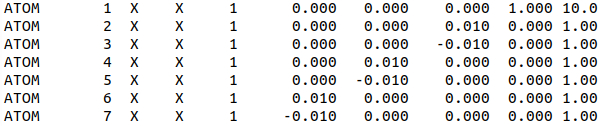
\includegraphics[scale = 0.5 ]{Images/valid_pqr.jpg}
    \caption{File UNITSPHERE\_DISC.pqr content.}
    \label{fig:valid_pqr}
\end{figure}

The domain is the cube $\Omega = [-32, 32]^3$, while the resulting molecular surface is a sphere of radius 10\AA, as schematically shown in Figure \ref{fig:valid_dom}, where the six particles with null charge have been neglected for simplicity, because they don't affect neither the exact and numerical solutions calculation nor the resulting molecular surface.

\begin{figure}[H]
    \centering
    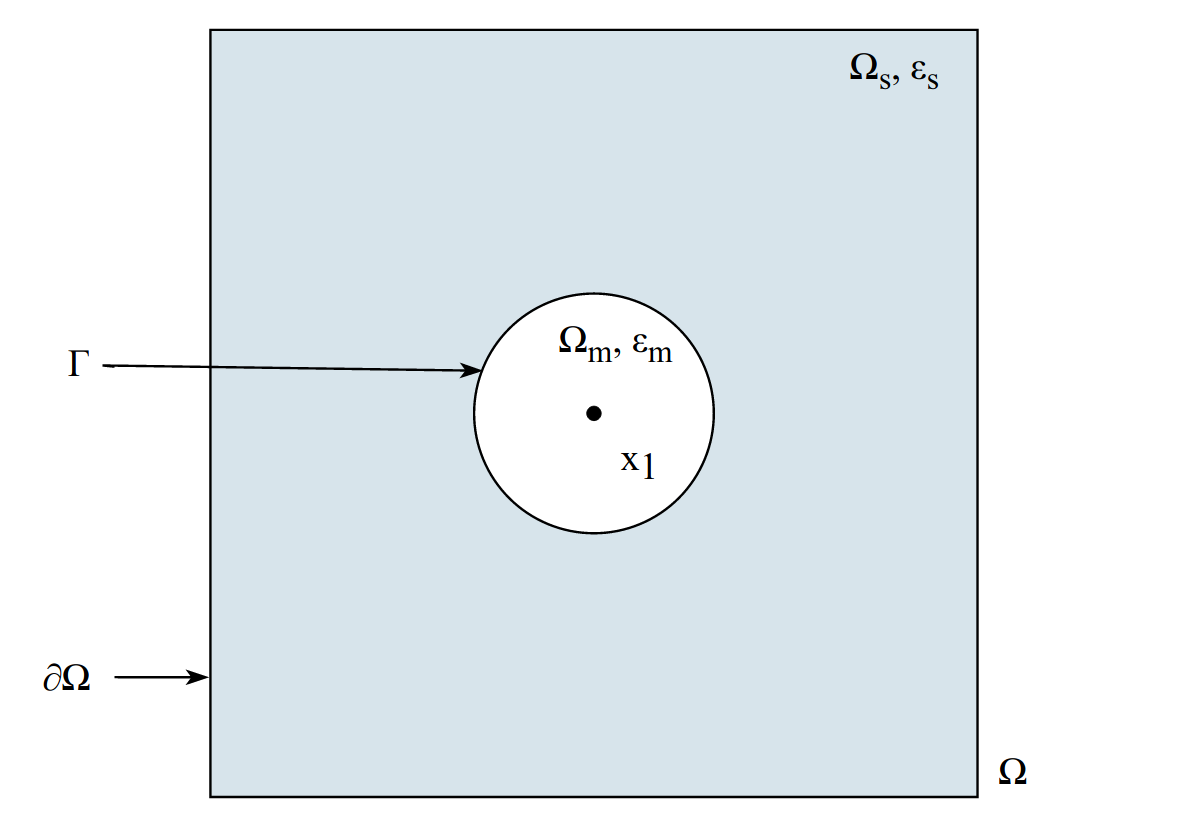
\includegraphics[width=0.5\textwidth]{Images/validat_dom.png}
    \caption{Schematic representation of the domain used for the validation tests.}
    \label{fig:valid_dom}
\end{figure}

\subsection{Test Case in a Homogeneous Dielectric}
The first test case was done to compare the exact solution with the one calculated with our code in a homogeneous dielectric. 
The problem geometry is the same reported in Figure \ref{fig:valid_dom}, but the distinction between $\Omega_m$ and $\Omega_s$ refers only to the molecular surface which separates the solvent and the solute, not to the dielectric coefficients. Indeed, they are assumed to be both equal to the vacuum permittivity in all the domain $\Omega$, which means $\varepsilon_m = \varepsilon_s = 1$. The unique charge is $q$ located at the axis origin, which coincides with the atom center $x_1$. \\
For this simple test case, we calculated the exact electrostatic potential $\varphi$ using Gauss's Law for the electric field. It states that the electric flux through any closed surface is proportional to the total electric charge enclosed by the surface, namely

\begin{equation}
    \oint_S E \cdot \mathbf{n}\ ds = \frac{q}{\varepsilon_0 \varepsilon_m},
    \label{eq:gauss_law}
\end{equation}

where $E$ indicates the electric field, $S$ is the closed surface containing the charge $q$ and $\mathbf{n}$ is the outward pointing unit normal at each point on the boundary. \\
In our case, the surface $S$ is a sphere of radius $r$ centered at the point charge $q$, which coincides with the proton charge. Exploiting the spherical symmetry, the electric field $E$ becomes a constant that can be taken out of the integral. Then, integrating the remaining quantities we obtain Coulomb's law

\begin{equation}
    E(r) = \frac{q}{4 \pi \varepsilon_0 \varepsilon_m r^2}.
    \label{eq:coulomblaw}
\end{equation}

Recalling the electrostatic potential definition 

\begin{equation*}
    E = - \nabla \varphi
    \label{eq:E_PHI}
\end{equation*}

and substituting Coulomb's law (\ref{eq:coulomblaw}), the equation we want to solve, in spherical coordinates, assumes the following expression

\begin{equation}
    - \frac{\partial \varphi(r)}{\partial r} = \frac{q}{4 \pi \varepsilon_0 \varepsilon_m r^2},  \mbox{\; \;} 0 < r < \infty.
    \label{eq:exact_eq}
\end{equation}

Integrating both sides of the above relation we obtain the following electrostatic potential 
\begin{equation}
    {\varphi}(r) = \frac{{q}}{4 \pi {\varepsilon}_0 \varepsilon_m r} + C,
    \label{eq:phi_exact}
\end{equation}

which is defined up to an additive constant. In order to find the value of the constant $C$, a position where the electrostatic potential is null have to be chosen. Assuming the potential null at infinity, namely
\begin{equation}
    \lim_{r \to \infty} {\varphi}(r) = 0,
\end{equation}

the constant $C$ is equal to 0 and the exact solution is given by the Coulomb potential

\begin{equation}
    {\varphi}(r) = \frac{{q}}{4 \pi {\varepsilon}_0 \varepsilon_m r}.
    \label{eq:test1_exact}
\end{equation}

For what concerns the numerical solution with our code, we calculated the potential by fixing the ionic strength to zero, so that also the $\kappa^2$ coefficient is zero and the solved equation coincides with (\ref{eq:exact_eq}). The boundary conditions were manually set as follows 

\begin{equation*}
    {\varphi}_{easy\_pbe}(r) = {\varphi}(r), \mbox{\; on } \partial \Omega.
\end{equation*}


The comparison between the numerical and theoretical solutions is reported in Figure \ref{fig:test1}. We calculated the easy\_pbe electrostatic potential using both a uniform grid and an adaptively refined grid. The former has with a discretization pass equal to 0.25\AA, the latter has minimum pass of about 0.03\AA\ and maximum pass 1\AA. This results in a uniform grid which is made of about 16,8 millions of cells, while the refined one contains about 2,6 octants.
Despite the large difference between the number of elements, in both cases the discrepancy from the exact solution is negligible.

\begin{figure}[H]
    \centering
    \subfloat[Uniformly refined Oct-tree grid of level 8.  \label{fig:test1_uni}]{
        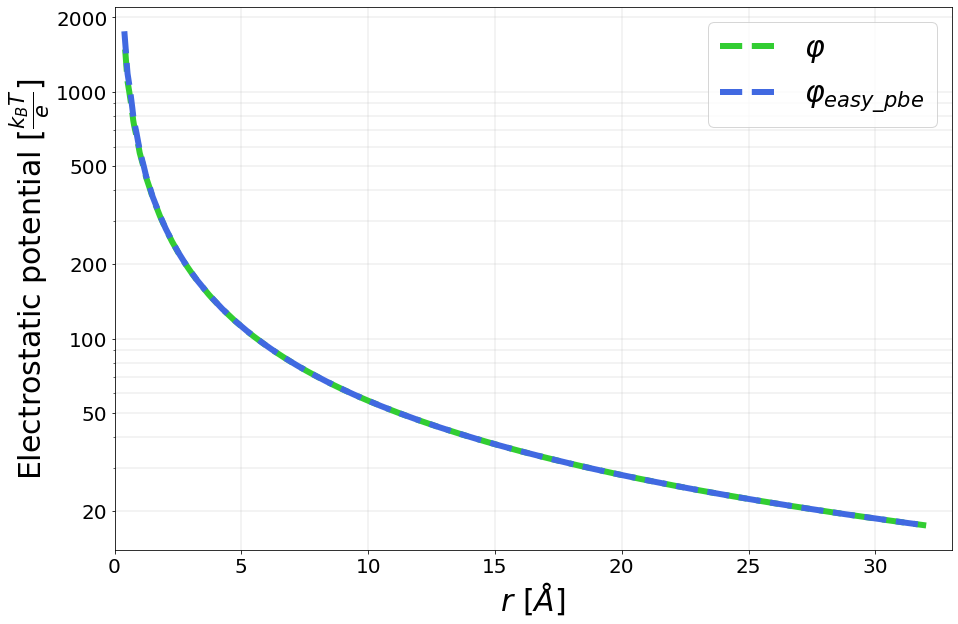
\includegraphics[scale=0.2381]{Images/test1_uni.png}
    }
    \quad
    \subfloat[Adaptive Oct-tree grid with maximum level of refinement equal to 11, minimum level equal to 6.\label{fig:test1_ref}]{
        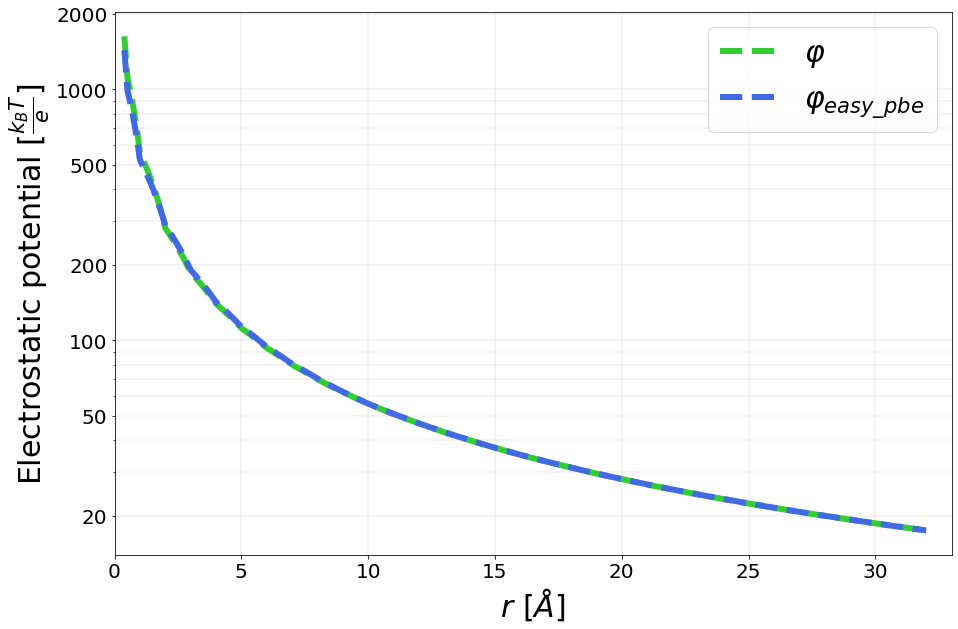
\includegraphics[scale=0.2381]{Images/test1_ref.png}
    }
    \caption[]{Exact solution (green) vs numerical solution (blue) calculated with easy\_pbe solver.}
    \label{fig:test1}
\end{figure}

In Figure \ref{fig:test1_error} the relative error of $\varphi_{easy\_pbe}$ calculated on the uniform grid nodes is represented. The curve rapidly drops to zero starting from the maximum value of about 17\%. Indeed, the relative error becomes less than 1\% from 1.5\AA\ and less than 0.1\% from 0.4\AA. The numerical solution becomes nodally exact in some point starting from 21\AA, in the solvent domain. 
The differences in the first part can be attributed to the imprecise geometry and to the source charge which is not precisely a point source for the solver. 
\begin{figure}[H]
    \centering
    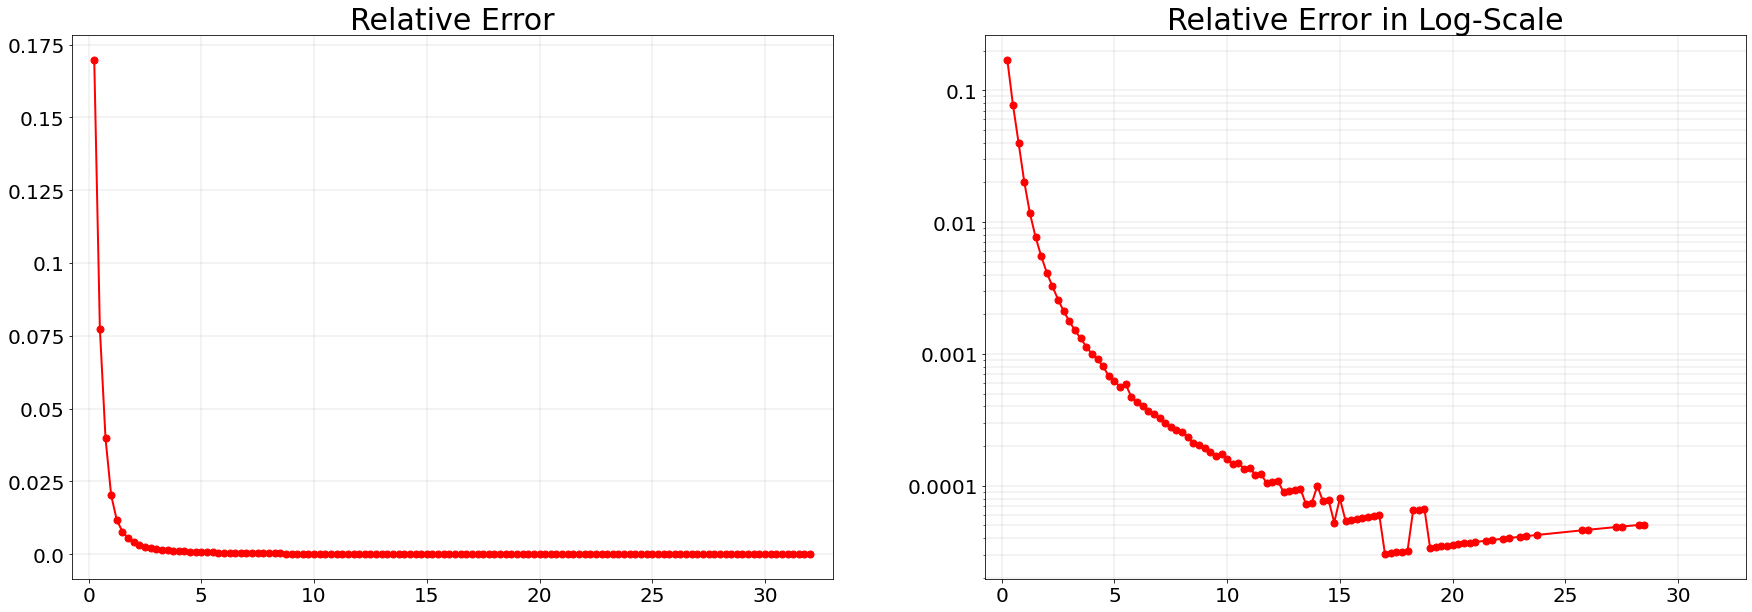
\includegraphics[scale=0.275]{Images/test1_error.png}
    \caption{Relative error of the electrostatic potential obtained using the uniform grid.}
    \label{fig:test1_error}
\end{figure}

\subsection{Test Case in a Non Homogeneous Dielectric}
In this second validation case we wanted to test if the electrostatic potential was correctly calculated when a dielectric discontinuity is present at the interface between the solvent and the solute. We compared the results obtained using the easy\_pbe solver with both the exact theoretical solution and the solution given by the Delphi solver, where the computational domain $\Omega_{Delphi}$ was $[-25,25]^3$ in both this and the following test cases. For easy\_pbe instead, the problem setting is the same introduced in the previous sections and reported in Figure \ref{fig:valid_dom}. Inside the sphere, we fixed the molecular relative permittivity coefficient $\varepsilon_m =1$, while outside the molecule the solvent permittivity constant is equal to $\varepsilon_s = 40$. Like in the previous test case, the ionic strength was fixed to zero, so that no reaction term is present in the equation. \\
Focusing on the region outside the molecule, the system of equations takes the form reported below

\begin{equation}
    \left\{
    \begin{aligned}
    & - \frac{1}{r^2}\ \frac{\partial}{\partial r}\ \Big( {\varepsilon}_0 \varepsilon_s r^2\ \frac{\partial {\varphi}_{out}}{\partial r} \Big) = 0, & \mbox{\;} r_s < r < \infty \\
     & - \Big( {\varepsilon}_0 \varepsilon_s\ \frac{\partial {\varphi}_{out}}{\partial r} \Big) \Big|_{r_s} = \frac{{q}}{4 \pi r_s^2} & \\
    & \lim_{r \to \infty} {\varphi}_{out}(r) = 0, &
    \end{aligned}
    \right.
    \label{eq:nonhomodiel_out}
\end{equation}

where $r_s$ is the radius of the molecular surface sphere. The first equation in (\ref{eq:nonhomodiel_out}) is the Poisson's equation where the rhs is equal to zero because no charge is present in the solvent. The second and third equation of the system are the boundary conditions of the problem. The first of the two is prescribed at the interface between the solvent and the molecule, the second assumes the potential equal to zero at infinity. The analytical solution of this problem is given by

\begin{equation}
    {\varphi}_{out}(r) = \frac{{q}}{4 \pi {\varepsilon}_0 \varepsilon_s r}.
    \label{eq:phi_out}
\end{equation}

Inside the molecular surface we can apply Gauss's Law for the electric field and use the electrostatic potential definition as before, which means that the equation to be solved is (\ref{eq:exact_eq}), with the corresponding solution (\ref{eq:phi_exact}). The constant $C$ can be found imposing the continuity of the electrostatic potential at the interface

\begin{equation}
    {\varphi}_{in}(r_s) = {\varphi}_{out}(r_s).
    \label{eq:bc_in}
\end{equation}

We obtain 
 
 \begin{equation}
    {\varphi}_{in}(r) = {\varphi}_{out}(r_s) + \frac{{q}}{4 \pi {\varepsilon}_0 \varepsilon_m r} \frac{(r_s - r)}{r_s}.
    \label{eq:phi_in}
\end{equation}

The exact electrostatic potential in all the domain $\Omega$ is the sum of the two local solutions (\ref{eq:phi_in}) and (\ref{eq:phi_out}) restricted to their region of interest

\begin{equation}
    {\varphi}(r) = {\varphi}_{in}(r)\chi_{_{\Omega_m}}(r) + {\varphi}_{out}(r)\chi_{_{\Omega_s}}(r).
    \label{eq:exact_unitsphere_disc}
\end{equation}

Then, we compared our result with the analytical solution and the numerical solution given by the Delphi solver. We imposed manually the analytical solution value at the boundary of the easy\_pbe potential, \emph{e.g.} ${\varphi}_{easy\_pbe}(r)|_{\partial \Omega} = {\varphi}(r)|_{\partial \Omega}$. In Delphi we don't have the possibility to set manually the desired value at the boundary, so we choose \emph{Coulombic} boundary conditions. This option gives an estimate of the potential at a certain distance. For the Poisson's equation, this value is equal to the potential generated by a point charge in a homogeneous dielectric with permittivity constant equal to $\varepsilon_s$, which is exactly ${\varphi}(r)|_{\partial \Omega}$. The results are reported in Figure \ref{fig:test2}, where $\varphi_{easy\_pbe}$ was calculated both on a uniform grid composed of about 16 millions of cells and a refined mesh with less than 6 millions of elements. Also in this case the graphs are very similar so that it is difficult to see the differences and the discontinuity at 10\AA\ is always well detected.

\begin{figure}[H]
    \centering
    \subfloat[Uniformly refined Oct-tree grid of level 8.  \label{fig:test2_uni}]{
        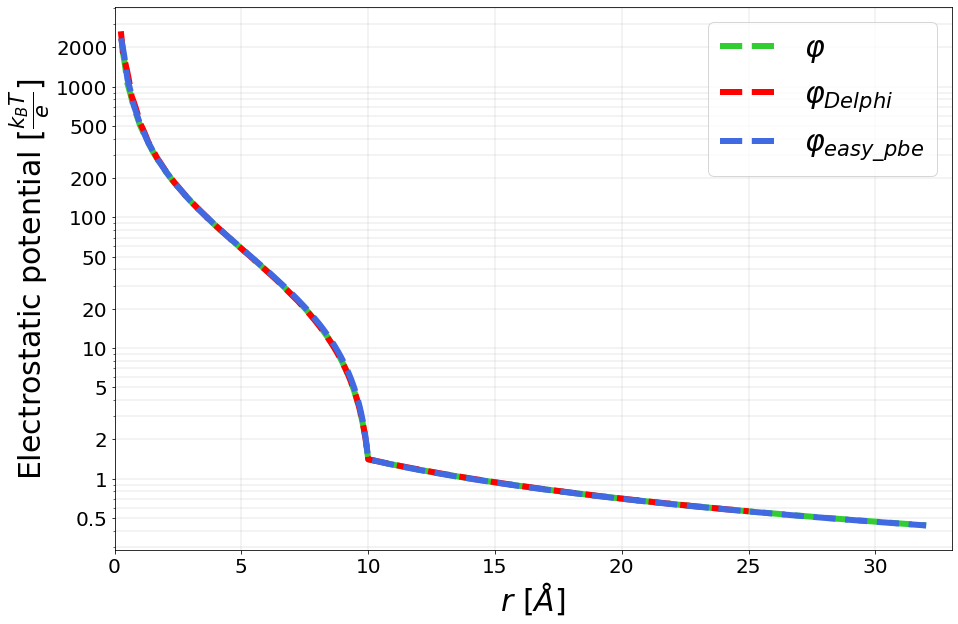
\includegraphics[scale=0.2381]{Images/test2_uni.png}
    }
    \quad
    \subfloat[Adaptive Oct-tree grid with maximum level of refinement equal to 11, minimum level equal to 6.\label{fig:test2_ref}]{
        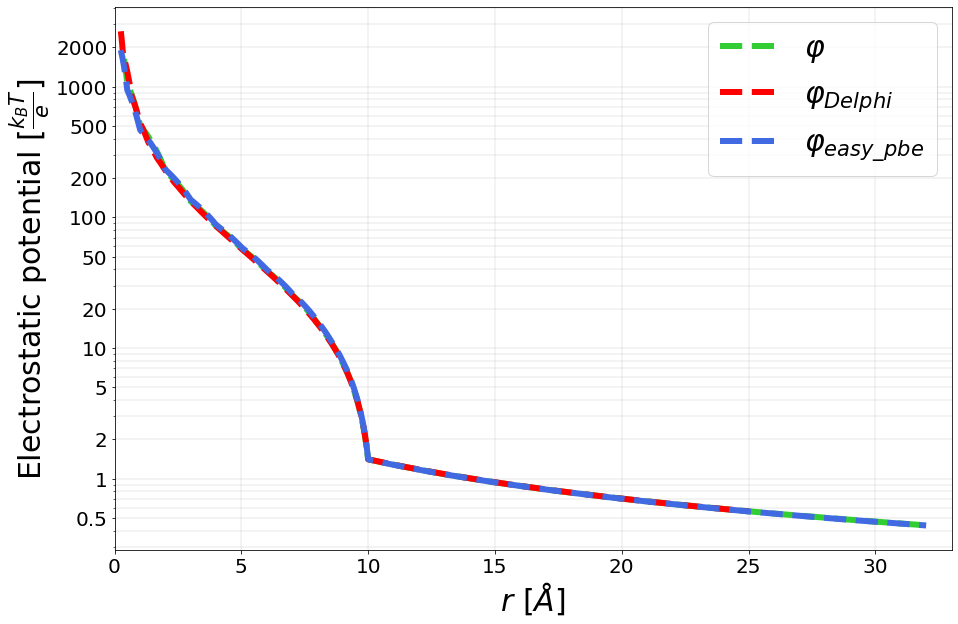
\includegraphics[scale=0.2381]{Images/test2_ref.png}
    }
    \caption[]{Comparison between exact solution (green), easy\_pbe solution (blue) and Delphi solution (red).}
    \label{fig:test2}
\end{figure}

 

\subsection{Test Case in a Non Homogeneous Dielectric with Reaction term}

In this last validation test the problem setting is the same of the previous validation case, where the two relative dielectric coefficients are $\varepsilon_m = 1$ and $\varepsilon_s = 40$. The only difference lies in the ionic strength, which is here fixed equal to the commonly accepted value of 0.145M. In this case the Poisson's equation becomes the PBE, where also the reaction term is present. We checked the correctness of our code by comparing the easy\_pbe potential with the analytical solution first, and then with Delphi's results. \\
Similar arguments to the ones made for the test without the reaction term can be done also in this situation. This means that, outside the molecule, the problem for the electrostatic potential becomes

\begin{equation}
    \left\{
    \begin{aligned}
    & - \frac{1}{r^2}\ \frac{\partial}{\partial r}\ \Big( {\varepsilon}_0 \varepsilon_s r^2\ \frac{\partial {\varphi}_{out}}{\partial r} \Big) + {\varepsilon}_0 \varepsilon_s\ \kappa^2 {\varphi}_{out} = 0, & \mbox{\;} r_s < r < \infty \\
     & - \Big( {\varepsilon}_0 \varepsilon_s\ \frac{\partial {\varphi}_{out}}{\partial r} \Big) \Big|_{r_s} = \frac{{q}}{4 \pi r_s^2} & \\
    & \lim_{r \to \infty} {\varphi}_{out}(r) = 0. &
    \end{aligned}
    \right.
    \label{eq:reaction_out}
\end{equation}

The solution translates into 

\begin{equation}
    \varphi_{out}(r) = \frac{{q}}{4 \pi {\varepsilon}_0 \varepsilon_s r} \frac{\mathrm{e}^{\kappa(r_s - r)}}{1 + \kappa r_s}.
    \label{eq:reac_phi_out}
\end{equation}

The problem in the solute is given by equation (\ref{eq:exact_eq}) coupled with (\ref{eq:bc_in}). The solution is given by (\ref{eq:phi_in}), with $\varphi_{out}(r_s)$ calculated from (\ref{eq:reac_phi_out}). The analytical solution is composed of the two contributions  (\ref{eq:exact_unitsphere_disc}). 

\bigskip
Numerically, we imposed ${\varphi}_{easy\_pbe}|_{\partial \Omega} = {\varphi}|_{\partial \Omega}$. The uniform and refined grids are characterized by the same number of cells reported for the previous test case and the results are close to the analytical solution as shown in Figure \ref{fig:test3_ex}.

\begin{figure}[H]
    \centering
    \subfloat[Uniformly refined Oct-tree grid of level 8.  \label{fig:test3_uni_ex}]{
        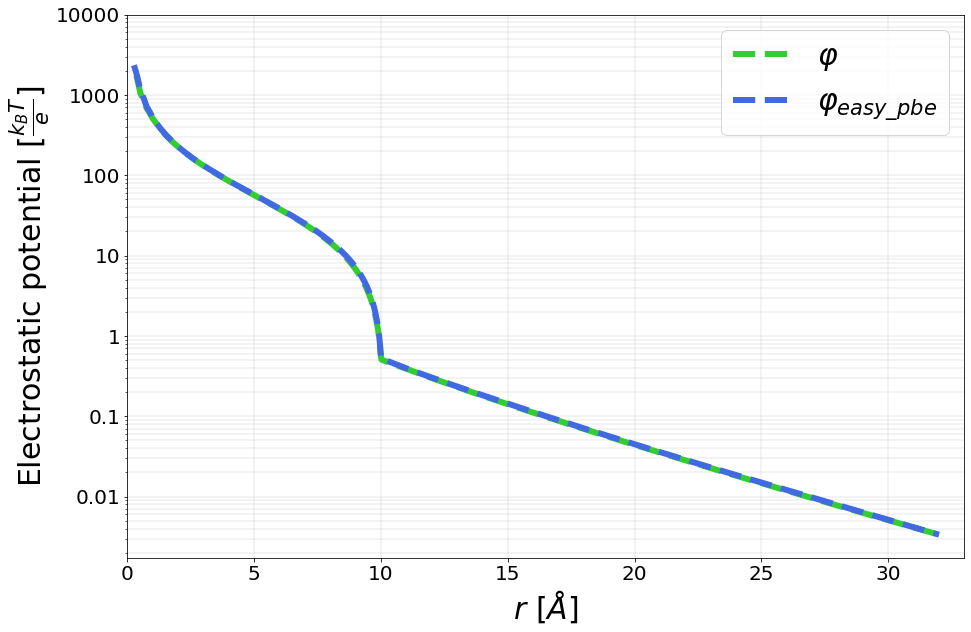
\includegraphics[scale=0.235]{Images/test3_uni_ex.png}
    }
    \quad
    \subfloat[Adaptive Oct-tree grid with maximum level of refinement equal to 11, minimum level equal to 6.\label{fig:test3_ref_ex}]{
        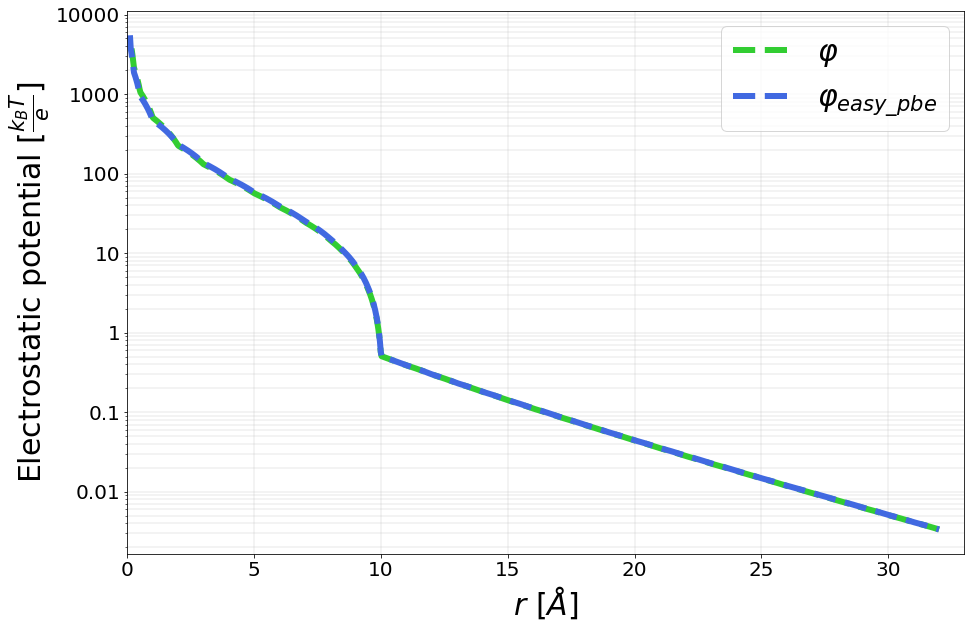
\includegraphics[scale=0.235]{Images/test3_ref_ex.png}
    }
    \caption[]{Exact solution (green) vs easy\_pbe solution (blue).}
    \label{fig:test3_ex}
\end{figure}

For this problem, the comparison with Delphi is less accurate because the Coulombic boundary conditions for the PBE do not coincide with the exact ones, but they are based on the Debye--H\"uckel theory that are more precise with higher ionic strength values. We choose homogeneous Dirichlet boundary conditions for our code, which are the ones chosen for the simulations where the exact value is not known a priori. The potentials obtained from these numerical simulations are shown in Figure \ref{fig:test3_del}. The differences between the two curves are more visible from about 20\AA\ to 25\AA, where the  $\Omega_{Delphi}$ boundary is located, while the trends are very similar in the other points.
At 32\AA, our solution drops to zero, as expected from the imposed BCs.

\begin{figure}[H]
    \centering
    \subfloat[Uniformly refined Oct-tree grid of level 8.  \label{fig:test3_uni_del}]{
        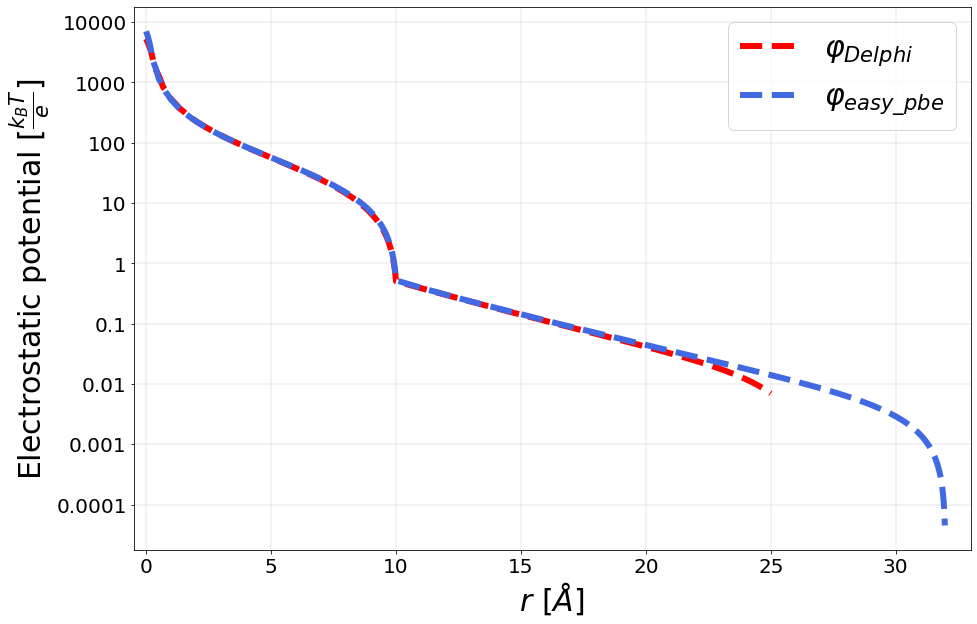
\includegraphics[scale = 0.233]{Images/test3_uni_del.png}
    }
    \quad
    \subfloat[Adaptive Oct-tree grid with maximum level of refinement equal to 11, minimum level equal to 6.\label{fig:test3_ref_del}]{
        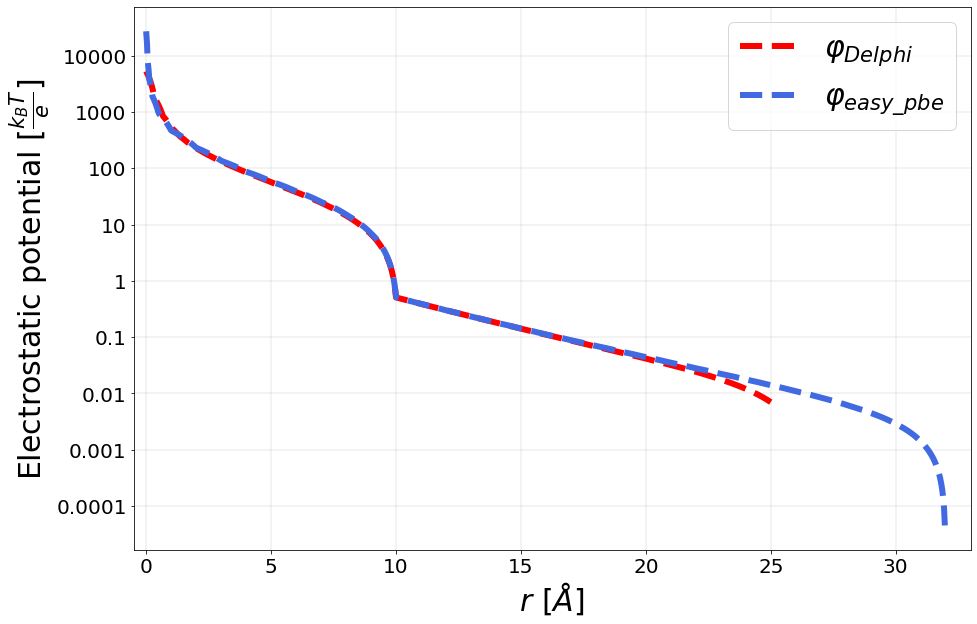
\includegraphics[scale = 0.233]{Images/test3_ref_del.png}
    }
    \caption[]{Delphi solution (red) vs easy\_pbe solution (blue).}
    \label{fig:test3_del}
\end{figure}

\section{Numerical Results on Real Molecules}
\label{sec:num_res}
Nowadays, the use of molecular electrostatics simulations in chemistry and biology is still an important tool. The main applications regard the protein folding and structural-based drug design, which, by making use of cutting-edge HPC techniques, can be applied to large and complex molecules. 
We tested our code with different molecules for different targets, whose main results are presented in the following sections. The structural data of the biological macromolecules are all taken from RCBS Protein Data Bank \cite{RCBS}.

\subsection{Crambin Test Case}
\label{sec:crambin}
The first protein used for testing our code is a plant seed protein called crambin \cite{1ccm, 1ccm2}. It is relatively small as it is composed of 327 atoms and a unique protein chain. We employed the crambin molecule in order to both evidence the main differences between the three molecular surface definitions presented in this thesis and compare the potential with the one calculated by Delphi. The simulations have been performed on the computing server GIGAT of the MOX lab of Politecnico di Milano (6 nodes, 12 Intel Xeon E5-2640v4 @ 2.40GHz, 120 cores, 64GB RAM per node, O.S. CentOS 7 interconnected by a dedicated Gigabit Ethernet), on 1 node and 8 processors. \\
In Figure \ref{fig:crambin} you can see the electrostatic potential at the surface using respectively Blobby surface (Figure \ref{fig:1ccmblobby}), Skin surface (Figure \ref{fig:1ccmskin}) and Connolly surface (Figure \ref{fig:1ccmses}). In the three examples, the domain extremes are the ones corresponding to the \emph{stretched} mesh option, in this case $\Omega = [-22.73, 25.085] \times [-27.01, 27.146] \times [-22.169, 22.309]$.

\begin{figure}[H]
    \centering
    \subfloat[Blobby with B = -2.5.\label{fig:1ccmblobby}]{
        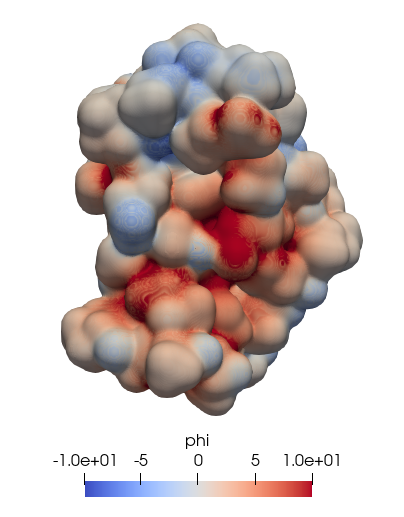
\includegraphics[scale=0.32]{Images/1ccm_blobby_3.png}
    }
    \quad
    \subfloat[Skin with s = 0.45.\label{fig:1ccmskin}]{
        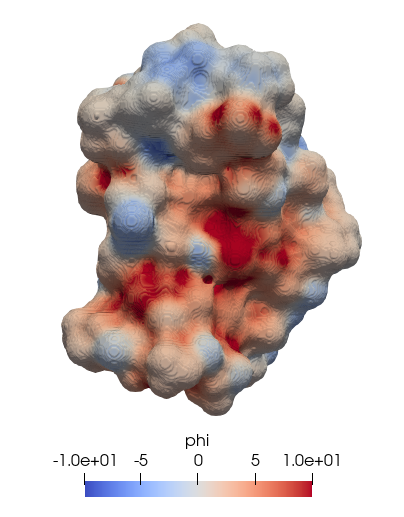
\includegraphics[scale=0.32]{Images/1ccm_skin.png}
    }
    \quad
    \subfloat[SES with probe radius 1.4\AA.\label{fig:1ccmses}]{
        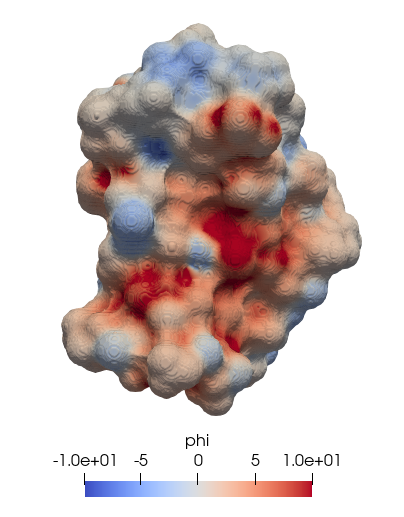
\includegraphics[scale=0.32]{Images/1ccm_ses.png}
    }
    \caption[]{Electrostatic potential at the surface for a crambin molecule using different surface representations.}
    \label{fig:crambin}
\end{figure}

Looking at the three shapes, the Blobby one is most recognizable, while 
the Skin and SES surfaces, characterized by an higher livel of detail, are very similar to each other. This can be explained recalling that the Blobby surface definition is based on the level-set method, while Skin and SES rely both on alpha-shapes. \\
The electrostatic potential values at the molecular surface seem to be qualitatively similar in all the three cases. To inspect better the results, we plotted $\varphi$ on a line passing through the center and parallel to the x axes, as shown in Figure \ref{fig:phi_x_surfs}. Notice that the line used for the extraction of the values is completely arbitrary and equivalent results can be obtained with other sampling choices. Also in this case the results given by the three surfaces are similar. The Skin and SES curves are extremely close one to the other, while the potential obtained with the Blobby surface presents some more evident discrepancies from the other two, especially inside the molecule. This is again attributable to the surface aspect, which affects the resulting grid and the numerical solution. 

\begin{figure}[H]
    \centering
    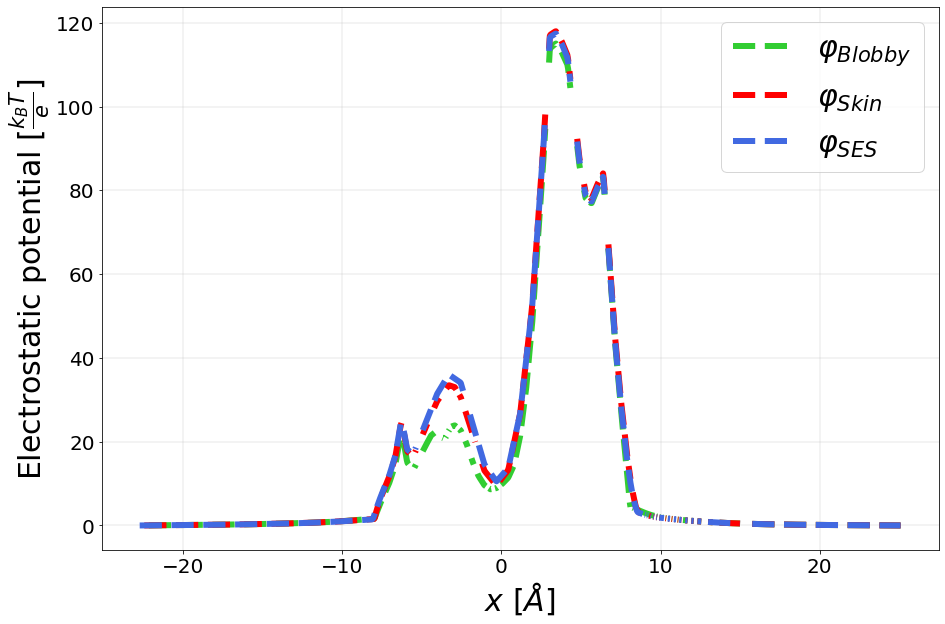
\includegraphics[scale = 0.3]{Images/1ccm_superfici_x.png}
    \caption{Electrostatic potential value for the crambin molecule over a line parallel to the x axes and passing through the center.}
    \label{fig:phi_x_surfs}
\end{figure}

 In table \ref{table:1ccm} we reported some useful information about the three simulations. The last two columns contain the number of cells corresponding to each test and the computational times for the principal operations made by the code:
\begin{itemize}
    \item Computation of the electrostatic potential (P);
    \item Creation of the markers (M);
    \item Adaptive refinement of the mesh (R).
\end{itemize}.

\noindent Both these aspects are comparable for the last two surfaces, while the Blobby one, which presents more elements, has the highest computational costs.

\begin{table}[H]
    \centering 
    \begin{tabular}{| c | c | c | c |}
    \hline
    \rowcolor{bluePoli!40}
     Surface type & min-max-uni level & Times & Number of mesh cells \T\B \\
    \hline 
     & & P: 47.3448 s &  \T\B \\
    \textbf{Blobby} & 2-9-5 & M: 64.404 s & 1334572  \T\B \\
     &  &  R: 154.745 s &  \T\B \\
    \hline
     &   & P: 44.529 s &   \T\B\\
    \textbf{Skin} &  2-9-5 & M: 5.750 s & 1218722 \T\B\\
     &  & R: 62.073 s &   \T\B\\
    \hline
     &  & P: 45.913 s &   \T\B\\
    \textbf{SES} & 2-9-5 & M: 5.668 s & 1206458 \T\B\\
    & & R: 61.610 s &   \B\\
    \hline
    \end{tabular}
    \\[10pt]
    \caption{Comparison between different molecular surfaces for crambin molecule. Min-max-uni level refer to minumum, maximum and initial uniform level of refinement of the surface. }
    \label{table:1ccm}
\end{table}

In order to obtain the same level of refinement at the surface, with a uniform mesh the number of elements would be higher than 134mln. This means that the adaptive refinement produces a saving of about 99,01\%, 99,09\% and 99,10\% for Blobby, Skin and SES respectively. \\\\
In order to validate our solution, we compared the results obtained using the SES surface with the one given by Delphi solver. The Delphi potential was computed on a uniform grid, in which each side of the cubic domain was divided into 200 elements. Since our code can actually divide each side of the mesh by powers of two, we set the starting refinement level to 8, which corresponds to 256 subdivisions, and performed just one refinement iteration. Then, we projected the Delphi solution over the resulting grid, whose extremes were fixed equal to Delphi's ones. The first column in Figure \ref{fig:delphi_vs_easypbe_1ccm} shows that the easy\_pbe and Delphi potential values are almost exactly superposed. \\
Then, we tried to compare the Delphi results with a more pronounced refinement. In this case the minimum level was fixed to 5, while the maximum level to 9. In Figure \ref{mesh_compare} the differences between this and the previous mesh results.

\begin{figure}[H]
    \centering
    \subfloat[minlevel = 8, maxlevel = 9.\label{fig:meshuni}]{
        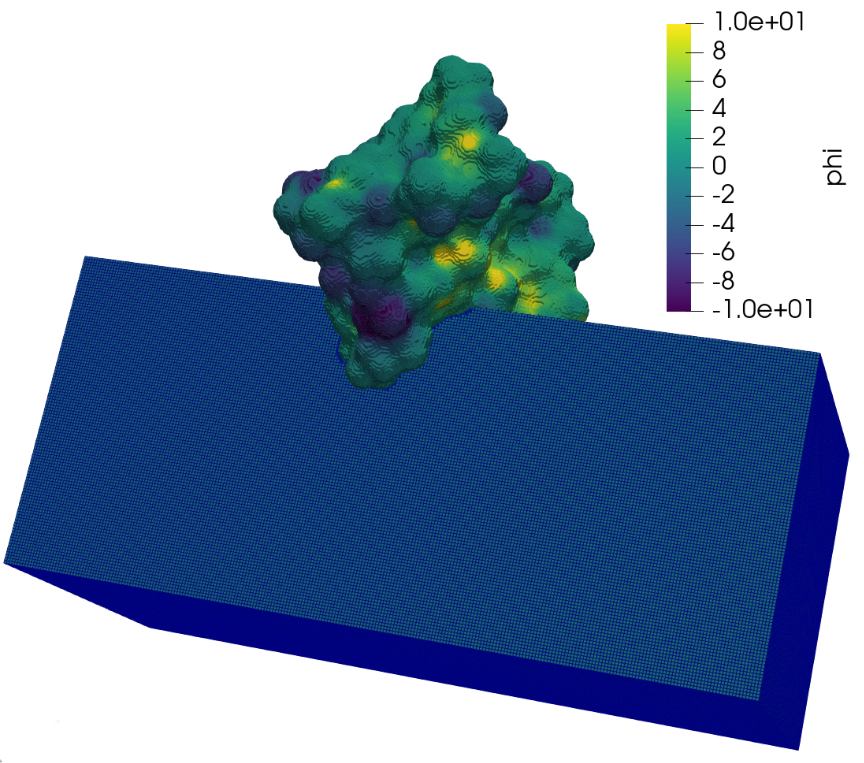
\includegraphics[scale=0.22]{Images/mesh_uni(1).jpg}
    }
    \quad
    \subfloat[minlevel = 5, maxlevel = 9. \label{fig:meshref}]{
        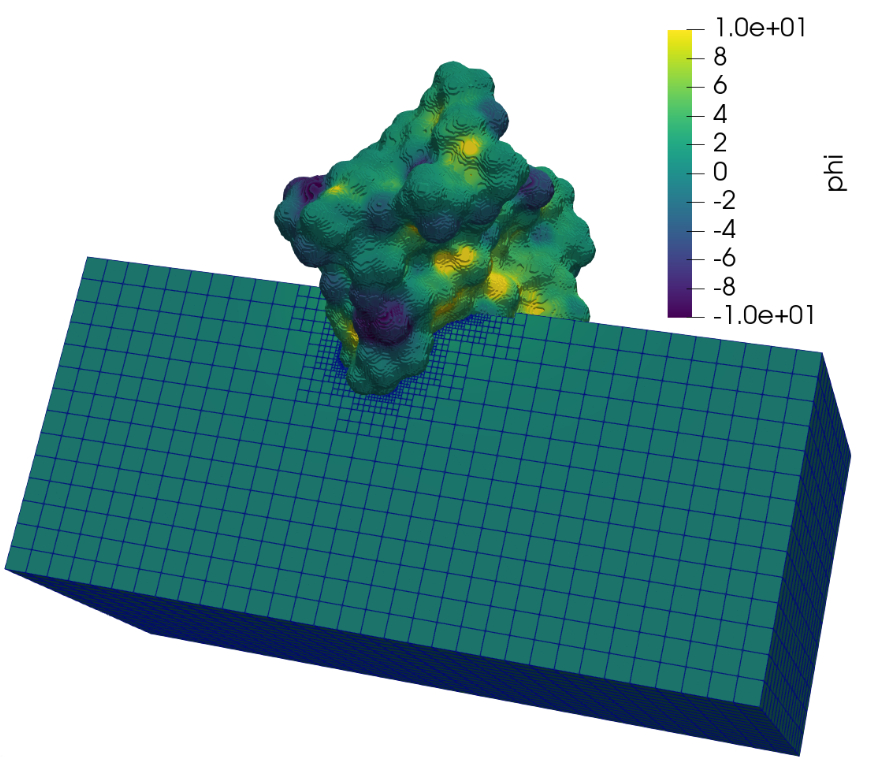
\includegraphics[scale=0.22]{Images/mesh_raffinata.jpg}
    }
    \caption[]{Comparison between an almost uniform mesh and a refined one.}
    \label{mesh_compare}
\end{figure}

The accuracy is still acceptable, even if there are some evident different in the potential mostly inside the molecular surface, as shown from column two in Figure \ref{fig:delphi_vs_easypbe_1ccm}.


\begin{figure}[H]
    \centering
    \subfloat[Potential values on the line parallel to x axes, with minlevel = 8, maxlevel = 9.   \label{fig:xr}]{
        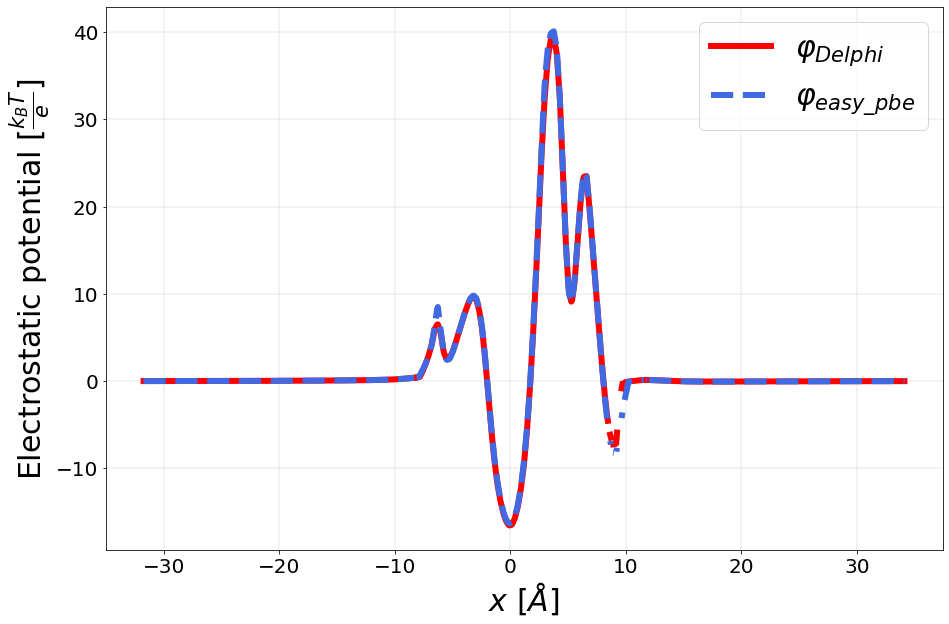
\includegraphics[scale=0.2381]{Images/xr_1ccm_easyvsdel.png}
    }
    \quad
    \subfloat[Potential values on the line parallel to x axes, with minlevel = 5, maxlevel = 9. \label{fig:yr}]{
        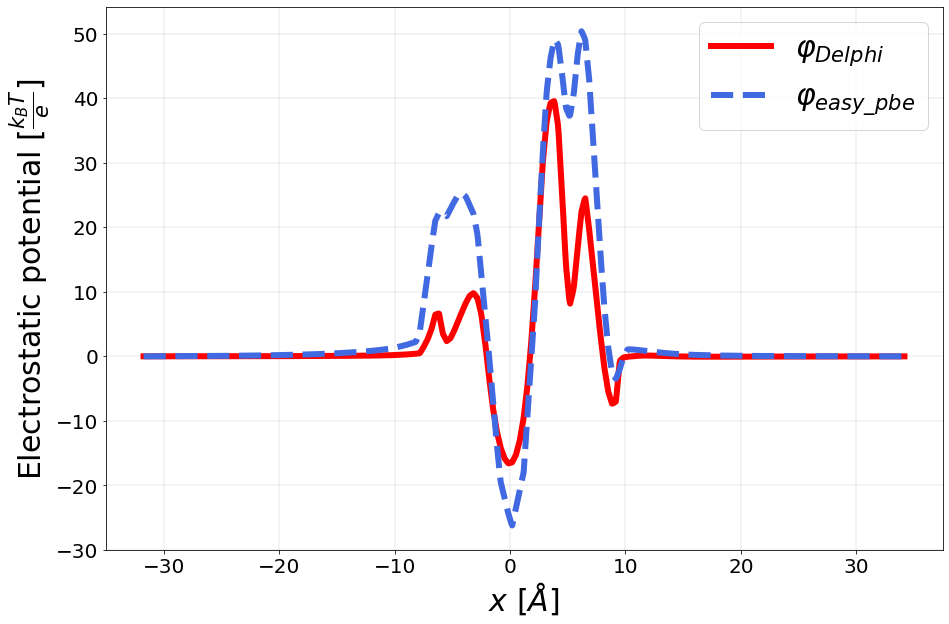
\includegraphics[scale=0.2381]{Images/xr_1ccm_easyvsdel_59.png}
    }
    \quad
    \subfloat[Potential values on the line parallel to y axes, with minlevel = 8, maxlevel = 9. \label{fig:yr}]{
        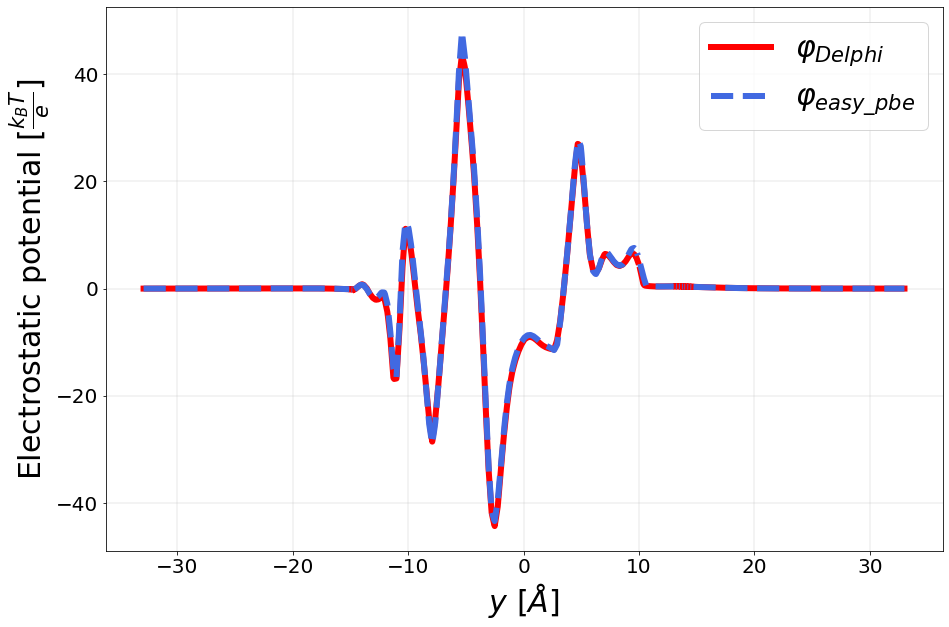
\includegraphics[scale=0.2381]{Images/yr_1ccm_easyvsdel.png}
    }
    \quad
    \subfloat[Potential values on the line parallel to y axes, with minlevel = 5, maxlevel = 9. \label{fig:yr}]{
        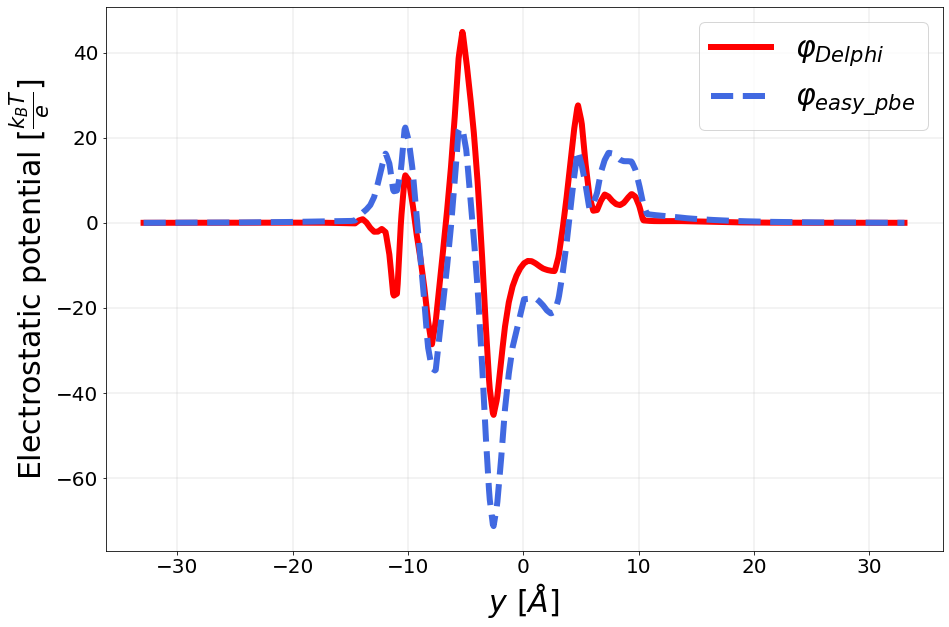
\includegraphics[scale=0.2381]{Images/yr_1ccm_easyvsdel_59.png}
    }
    \quad
    \subfloat[Potential values on the line parallel to z axes, with minlevel = 8, maxlevel = 9. \label{fig:zr}]{
        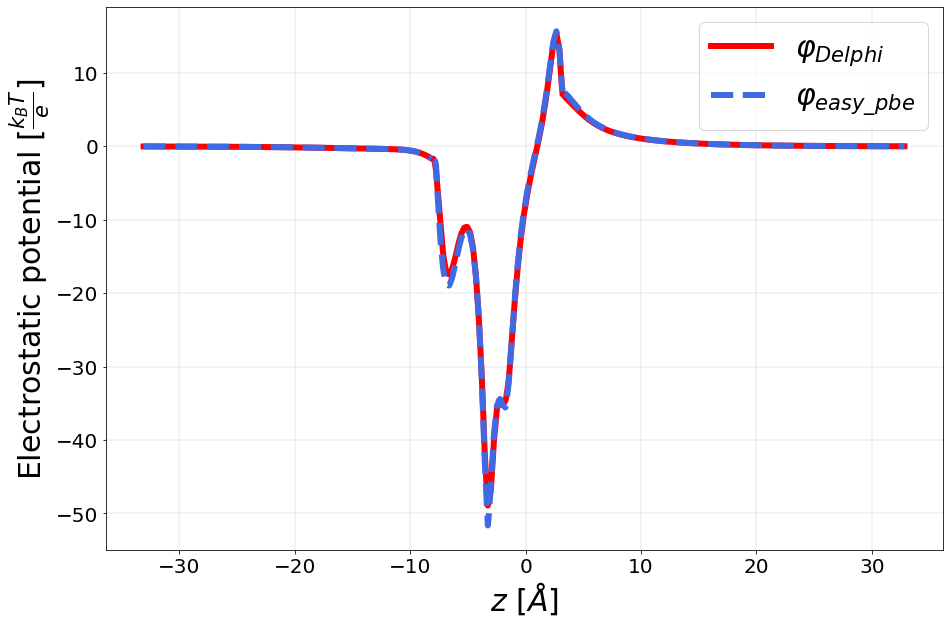
\includegraphics[scale=0.2381]{Images/zr_1ccm_easyvsdel.png}
    }
    \quad
    \subfloat[Potential values on the line parallel to z axes, with minlevel = 5, maxlevel = 9. \label{fig:yr}]{
        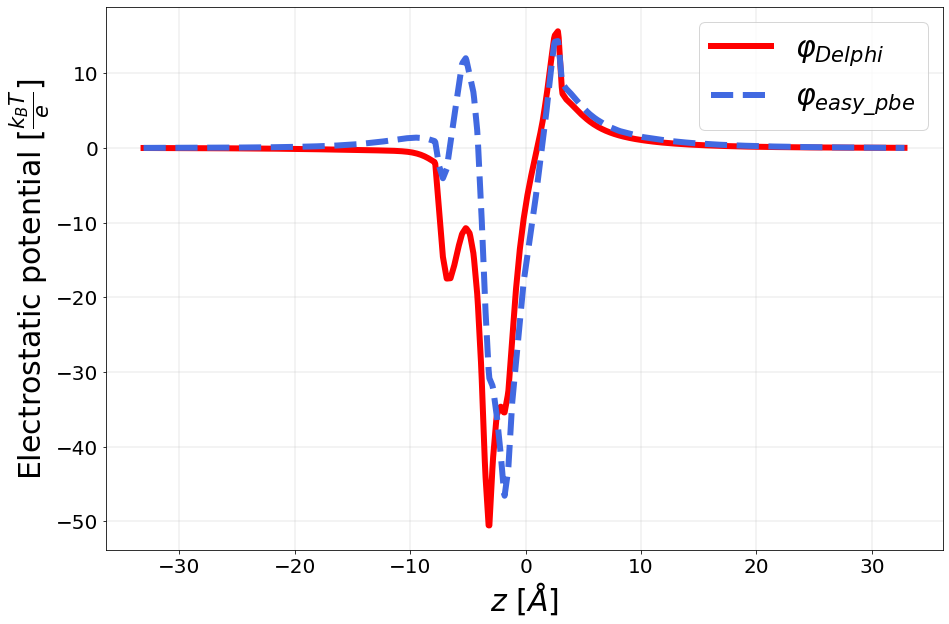
\includegraphics[scale=0.2381]{Images/zr_1ccm_easyvsdel_59.png}
    }
    \caption[]{Delphi and easy\_pbe potential values sampled on specific lines parallel to one axis and passing through the center of the domain.}
    \label{fig:delphi_vs_easy_graphs}
\end{figure}

Focusing on the potential values at the surface, shown in Figure \ref{fig:delphi_vs_easypbe_1ccm}, the results are comparable even if the last one is obtained with a mesh composed of about  one tenth of cells of Delphi. 

\begin{figure}[H]
    \centering
    \subfloat[Delphi solution.  \label{fig:delphi_1ccm}]{
        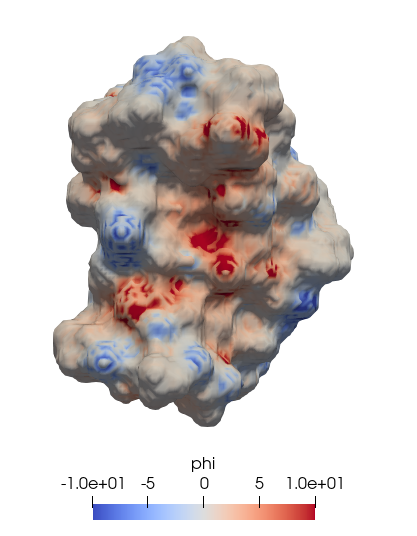
\includegraphics[scale = 0.32]{Images/delphi_1ccm.png}
    }
    \quad
    \subfloat[easy\_pbe solution with parameters minlevel = 8, maxlevel = 9, surface = SES with 1.4\AA\ probe radius.\label{fig:easypbe_1ccm}]{
        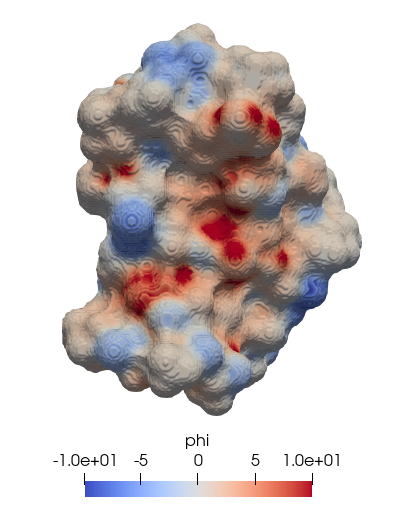
\includegraphics[scale = 0.32]{Images/easypbe_1ccm_89.png}
    }
    \quad
    \subfloat[easy\_pbe solution with parameters minlevel = 5, maxlevel = 9, surface = SES with 1.4\AA\ probe radius.\label{fig:easypbe_1ccm_59}]{
        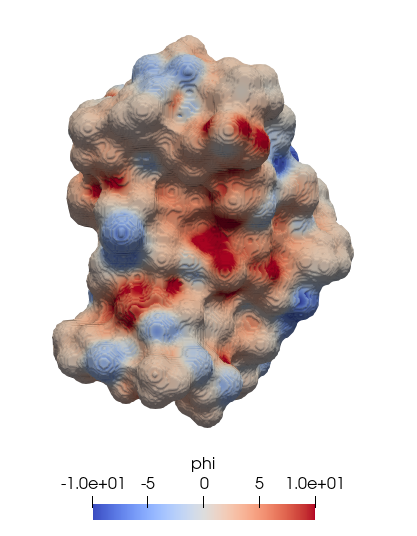
\includegraphics[scale = 0.32]{Images/easypbe_1ccm_59.png}
    }
    \caption[]{Crambin electrostatic potential at the surface computed with Delphi and easy\_pbe.}
    \label{fig:delphi_vs_easypbe_1ccm}
\end{figure}


\subsection{Parallel Scaling Test}
\label{sec:scaling}
In this section, we present the results of parallel scalability tests that have been performed again on the computing server GIGAT
of the MOX lab of Politecnico di Milano. We choose the nerve growth factor, whose structure can be seen in Figure \ref{fig:4xpj}, which is an important protein that is involved in a variety of physiological processes in cell survival, differentiation, proliferation and maintenance \cite{4xpj, 4xpj2}. It is composed of a unique protein chain and 1750 atoms. 


\begin{figure}[H]
    \centering
    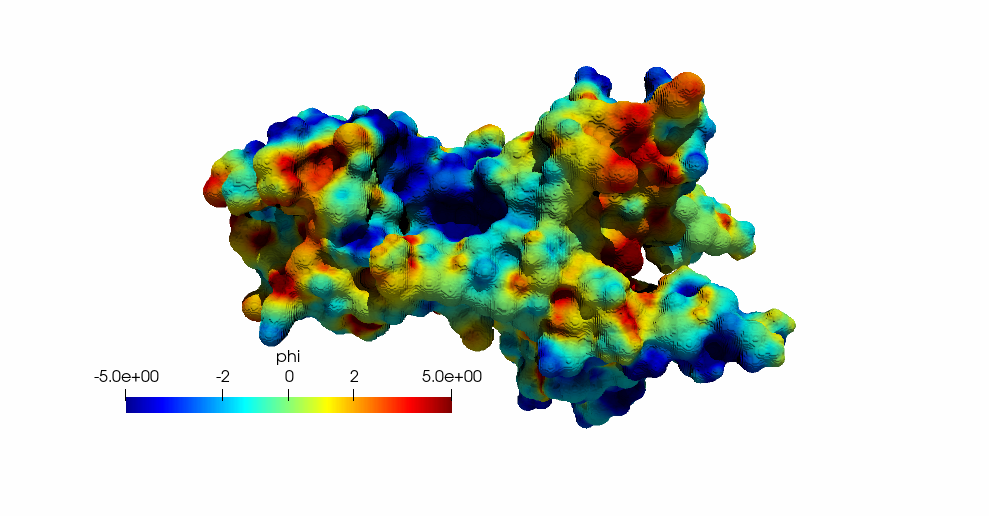
\includegraphics[width=0.8\textwidth]{Images/4xpj.png}
    \caption{Electrostatic potential value calculated at the surface of crystal structure of Nerve growth factor.}
    \label{fig:4xpj}
\end{figure}

The results of parallel scalability tests are reported in Figure \ref{fig:scaling}. The trend of the curves is very close to the linear line up to 8 processors, after that, the distance with the linear curve increases, but the computational time saving is still satisfying. As expected, the direct solver is slower than the iterative one, as Figure \ref{fig:linsol_speedup} shows.      



\begin{figure}[H]
    \centering
    \subfloat[\label{fig:geom_speedup}]{
        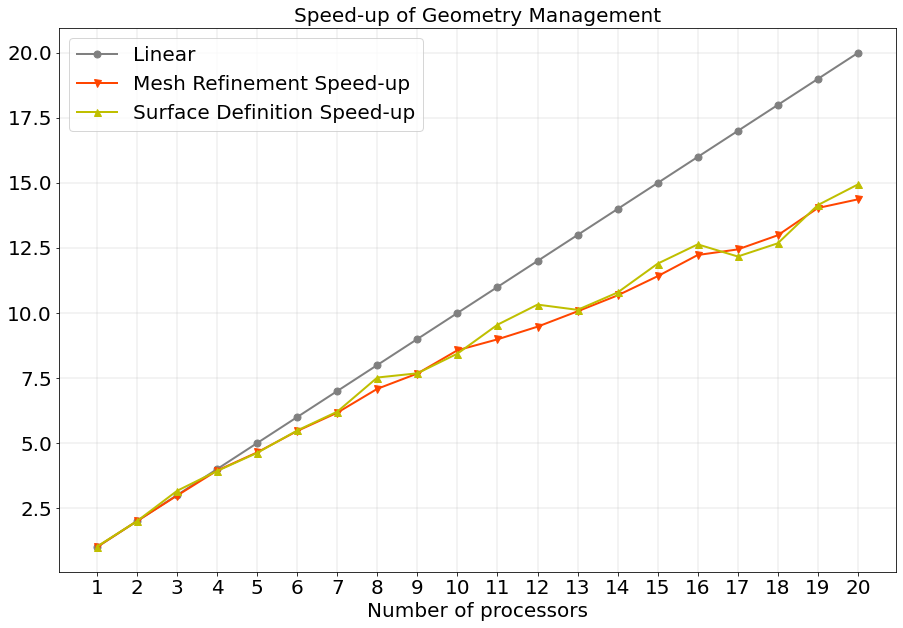
\includegraphics[scale=0.25]{Images/geometry_speedup.png}
    }
    \quad
    \subfloat[\label{fig:linsol_speedup}]{
        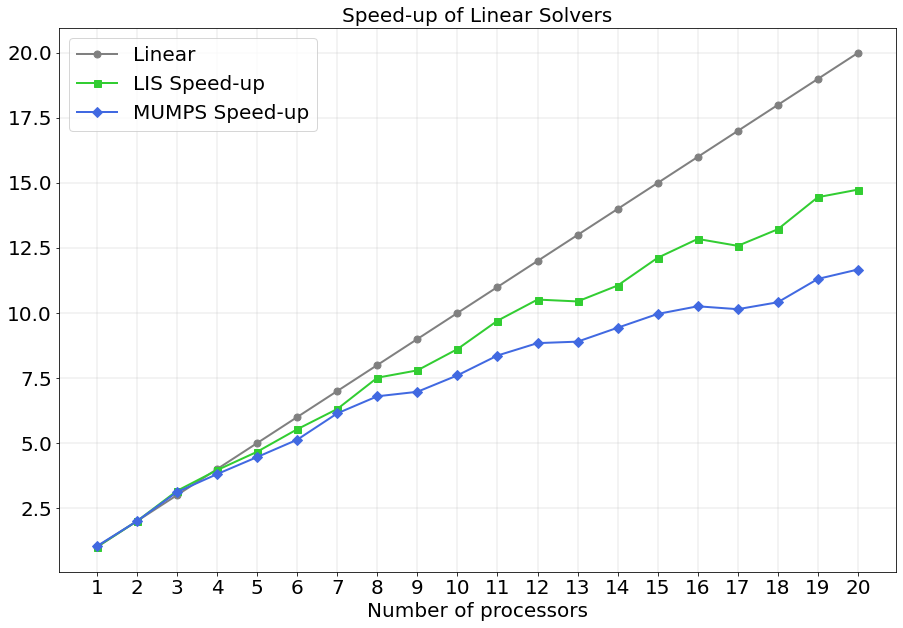
\includegraphics[scale=0.25]{Images/linsolv_speedup.png}
    }
    \caption[]{Figures (a) and (b) refer respectively to the speed-up of the Geometry Management and Linear Solvers using 1 node and 1--20 processors.}
    \label{fig:scaling}
\end{figure}


\section{Concluding Remarks and SARS-CoV-2 Spike Protein Simulation}
\label{sec:spike}
The role of electrostatics in bio-molecular recognition is prominent, this is due to the features of electrostatic interactions both at long and short distances. Indeed, long range electrostatic interactions impact both on general repulsion/attraction of same and differently charged molecules, but also on the time that two biomolecules stay in close proximity, allowing them to find the most complementary conformations \cite{roc1}. Short range electrostatics is also extremely important, since it helps achieve the specificity that is necessary for the correct functioning of biochemical signalling. Its contribution to solvation is the third element which makes electrostatics so relevant in this field. \\
The Poisson Boltzmann equation is routinely used to estimate the role of electrostatics and desolvation to molecular binding, as well as to pKa shifts in titratable residues and in many other situations. It proved able to pinpoint molecular determinants of protein-protein interaction specificity \cite{roc2} as well as the effects of shape in protein-DNA interaction
\cite{roc3}. \\
For such reasons, Poisson-Boltzmann calculations, may deserve to be considered  one of the enabling 
technologies for developing automatic strategies for drug discovery or drug repurposing.

To test the applicability of our solver on molecular structures of actual interest for
applications we ran  {\tt easy\_pbe} simulations on
two molecules that are clearly relevant targets for this sort of studies, in particular the spike
protein of two different strains of the SARS-CoV-2 virus, first strain \cite{ 6vyb, 6vyb2} 
versus the Omicron variant \cite{7tb4, 7tb42}. 
Results reported in Figure~\ref{fig:covid} were obtained using SES surface and took about 4 and 3 hours respectively on the computing server GIGATLONG of the MOX lab of Politecnico di Milano, using 20 processors. The times are divided in the following way:
\begin{itemize}
    \item Between 59-60\% for the refinement and coarsening steps,
    \item between 39-40\% for the calculus of the electrostatic potential,
    \item the remaining time for the markers computation and the export of the calculated quantities, mesh included.
\end{itemize}


\begin{figure}[H]
    \centering
    \subfloat{
        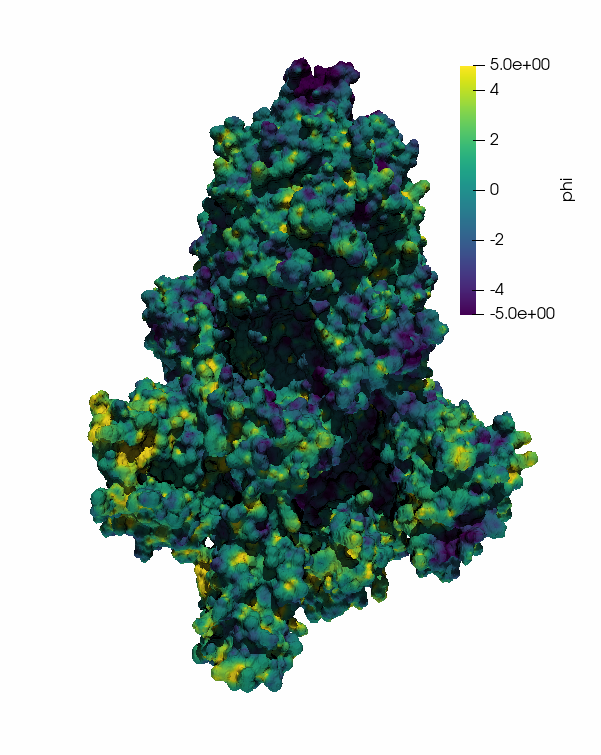
\includegraphics[scale=0.3]{Images/covid.png}
    }
    \quad
    \subfloat{
        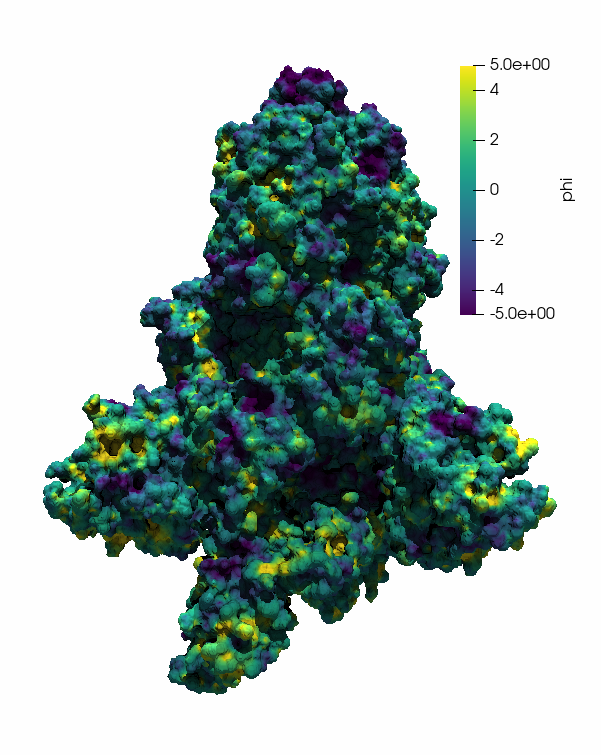
\includegraphics[scale=0.3]{Images/omicron.png}
    }
    \caption[]{SARS-CoV-2, spike protein,  ectodomain structure open state (left), 
    Omicron variant of concern (right).}
    \label{fig:covid}
\end{figure}

%-----------------------------------------------------------------------------
% CONCLUSION
%-----------------------------------------------------------------------------

%-----------------------------------------------------------------------------
% BIBLIOGRAPHY
%-----------------------------------------------------------------------------
\bibliography{bibliography.bib}

\appendix
\section{\texttt{easy\_pbe} user reference}
\label{App_A}
This appendix contains the instructions on how to compile and use the code and  visualize the outputs. \\
The implemented code can be found inside the repository: \url{https://github.com/carlodefalco/easy_pbe}, and its structure is schematically reported in Figure \ref{code_structure}. 

\begin{figure} [H]
\centering
\tikzstyle{every node}=[draw=black,thick,anchor=west]
\tikzstyle{repo}=[draw=bluePoli!150,fill=bluePoli!30]
\tikzstyle{folder}=[draw=bluePoli!100,fill=bluePoli!15]
\tikzstyle{file}=[draw=bluePoli!60,fill=white]
\begin{tikzpicture}[scale = 0.9, font = \small, %
  grow via three points={one child at (0.5,-0.7) and
  two children at (0.5,-0.7) and (0.5,-1.4)},
  edge from parent path={(\tikzparentnode.south) |- (\tikzchildnode.west)}]
  \node [repo] {easy$\_$pbe}
    child { node [folder] {data}
    child {node [file] {*.pqr}}
    child {node [file] {options.pot}}
    }	
    child [missing] {}	
    child [missing] {}
    child { node [folder] {include}
    child {node [file] {GetPot, GetPot.hpp, GetPot.cpp}}
    child {node [file] {json.hpp}}
    child {node [file] {pb\_class.h}}
    child {node [file] {raytracer.h}}
    child {node [file] {serialize.h}}
    }
    child [missing] {}
    child [missing] {}	
    child [missing] {}
    child [missing] {}	
    child [missing] {}
    child { node [folder] {src}
    child {node [file] {Makefile}}
    child {node [file] {pb\_class.cpp}}
    child {node [file] {poisson\_boltzmann.cpp}}
    child {node [file] {raytracer.cpp}}
    };
\end{tikzpicture} 
\caption{Repository structure scheme with both folders and files.}
\label{code_structure}
\end{figure}
The repository contains three directories. Inside the folder \texttt{data} two kind of files are included: the \texttt{option.pot} file, in which the user can set the parameters for the simulation, and some \texttt{.pqr} files with the molecule information. The \texttt{include} and \texttt{src} directories respectively contain the header and source files of the code. Inside the \texttt{src} folder the main function \texttt{poisson\_boltzmann.cpp} and the \texttt{Makefile}, necessary for the compilation, can be found.

\subsection{Installation}
The direct dependencies of the code are \texttt{bim++} and \texttt{NanoShaper}, while Paraview and \texttt{octave} are necessary for the post-processing operations. \\
For the compilation, a \texttt{local\_settings.mk} file must be created in order to add or modify, accordingly to the user necessities, the compilation options present inside \texttt{Makefile}, and then the following command must be executed 
\begin{code}
make
\end{code}

\subsection{Input files}
The code takes as input two files:
\begin{itemize}
    \item \texttt{options.pot} file, containing the parameters for the simulation;
    \item .pqr file.
\end{itemize}
\bigskip
The .pqr file format is a modification of the .pdb format, which is used for the description of the 3D structure of the molecules of the Protein Data Bank. The correct .pqr format can be generated starting from the .pdb format using the PDB2PQR tool (\url{https://server.poissonboltzmann.org/pdb2pqr}) and selecting TYL06 as output naming scheme with the \emph{whitespaces} option activated together with the default ones. Inside a .pqr file all the information about the studied molecules can be found. In Figure \ref{fig:pqr_example} the first lines of the crambin molecule .pqr file are reported as an example of its content. 

\begin{figure}[H]
    \centering
    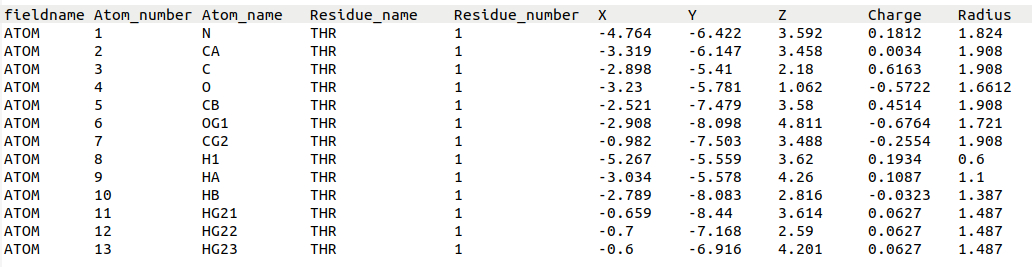
\includegraphics[scale = 0.4]{Images/pqr.jpg}
    \caption{First lines of 1CCM.pqr file.}
    \label{fig:pqr_example}
\end{figure}

The \texttt{fieldname} corresponds to a string which specifies the type of the PQR entry, it can be either ATOM or HETATM. The \texttt{Atom\_number} and \texttt{Atom\_name} are respectively an integer with the index of each atom and a string containing its name, while the following two fields regards the residue. The remaining columns are the most important because they contain the information for the electrostatic potential computation: the atomic coordinates of the atom center (expressed in \AA), the charge (expressed in electrons unit) and the atom radius (expressed in \AA). \\

An example of option file can be seen in Figure \ref{fig:pot_example}. 

\begin{figure}[H]
    \centering
    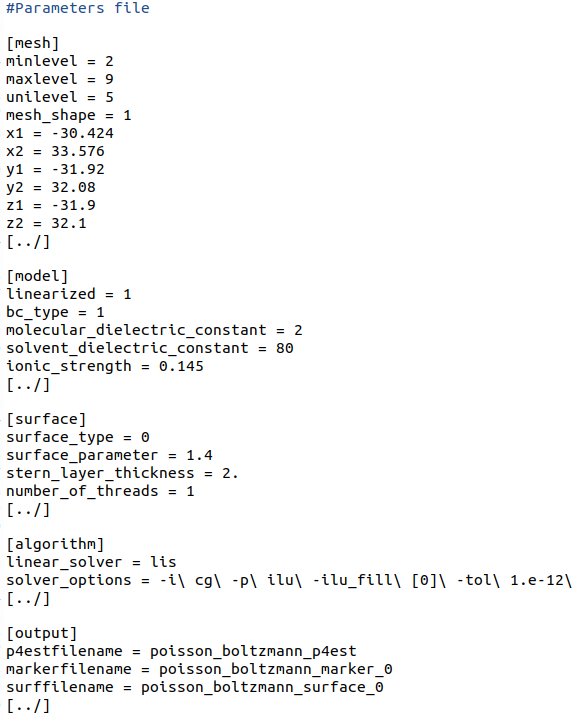
\includegraphics[scale = 0.4]{Images/pot.jpg}
    \caption{Example of \texttt{options.pot} file.}
    \label{fig:pot_example}
\end{figure}
Below the description of the parameters is reported.

Mesh options:
\begin{itemize}
    \item maxlevel: maximum level for the mesh refinement, root assumed level 0. 
    \item minlevel: minimum level for the mesh refinement.
    \item unilevel: level chosen for the initial uniform refinement of the mesh.
    \item mesh shape: it can be \emph{cubic} (option 0), \emph{stretched} (option 1) or \emph{manually set} (option 2). Consider for instance the problem domain
    \begin{equation*}
        \Omega = [x_{min}, x_{max}] \times [y_{min}, y_{max}] \times [z_{min}, z_{max}]
    \end{equation*}
    With \emph{cubic} option, the list of all the atoms inside the examined molecule is scrolled in order to find the maximum (minimum) coordinate value without distinguishing among the three axis directions. Then the right (left) domain extremes of each interval in $\Omega$ are set equal to this value summed (subtracted) to six times the maximum radius among all the atoms of the chosen molecule. In this way the min and max values of each interval are the same along the coordinates. \\
    For the \emph{stretched} option instead, the maximum (minimum) coordinate value is searched separately in every direction, so that in general $x_{min} \neq y_{min} \neq z_{min}$ and $x_{max} \neq y_{max} \neq z_{max}$. \\
    The user can also decide to set the domain coordinates explicitly by selecting the \emph{manual setting} and filling the corresponding spaces with the desired domain vertex coordinates. 
\end{itemize}
\bigskip
Model parameters:
\begin{itemize}
    \item linearized: 1 for solving the \emph{linearized} PBE, the only available up to now.
    \item bc\_type: 0 for homogeneous Neumann, 1 for homogeneous Dirichlet.
    \item molecular\_dielectric\_constant: relative permittivity constant of the molecule.
    \item solvent\_dielectric\_constant: relative permittivity constant of the solvent.
    \item ionic\_strength: $I$ expressed in molar concentration. 
\end{itemize} 
\bigskip
\texttt{NanoShaper} surface parameters:
\begin{itemize}
    \item surface\_type:
    \begin{itemize}
        \item 0 for SES (or Connolly surface);
        \item 1 for Skin surface;
        \item 2 for Blobby surface.
    \end{itemize}
    \item surface\_parameter:
    \begin{itemize}
        \item SES probe radius (default value 1.4\AA).
        \item Skin surface parameter $s \in (0,1)$. The default value is 0.45, which corresponds to a surface very similar to the SES one. If $s = 1$, it corresponds to the convex hull, if $s = 0$ it coincides with the Van der Waals surface. 
        \item Blobby parameter B (default value -2.5, not too far from SES). 
    \end{itemize}
    \item stern\_layer\_thickness:  (not yet available for \texttt{NanoShaper} API).
    \item number\_of\_threads: set the available threads for \texttt{NanoShaper} surface computation. 
\end{itemize}
\bigskip
Algorithm options:
\begin{itemize}
    \item linear\_solver: the user can decide to use either \texttt{mumps} direct solver, or \texttt{lis} iterative solver.
    \item solver\_options: only for the iterative solver, see \texttt{lis} manual \cite{lis_manual} for the complete list of available options, \emph{e.g.} solvers, preconditioners, tolerance, etc.  
\end{itemize}
\bigskip
Output options: arbitrary names for the creation of the output files.

\subsection{Launching Simulations from the Command Line}
To run the code in serial, using the default \texttt{options.pot} file and the 1CCM.pqr file, the necessary commands are
\begin{code}
mkdir results
cd results
../poisson_boltzmann 
\end{code}
 
To run in parallel with MPI, change the last line with
\begin{code}
mpirun -np <number of processes> ../poisson_boltzmann
\end{code}
with \texttt{processors\_number} equal to the desired number of processors. \\
To select a different option file add the following option
\begin{code}
--potfile /your/folder/<file name>.pot
\end{code}
While to change the input molecule add the following option
\begin{code}
--pqrfile /your/folder/<file name>.pqr
\end{code}

\subsection{Post-processing of Output Files}
The user can use the \texttt{octave} script called \texttt{export.m} and 
distributed with \texttt{bimpp} (it is located in the  folder \texttt{script/m})
for the post-processing. When the user adopts the default names for the files, it 
can write the following command line for the creation of a .vtu file that can be 
opened using Paraview. 

\begin{code}
export_tmesh_data ('poisson_boltzmann_surface_%1.1d_%4.4d',
                    {'poisson_boltzmann_surface_%1.1d_%4.4d', 'phi_%1.1d_%4.4d', 
                    'rhs_%1.1d_%4.4d', 'rho_%1.1d_%4.4d'}, {'surface', 'phi', 'rhs', 'rho'},
                    {'poisson_boltzmann_marker_%1.1d_%4.4d', 'epsilon_%1.1d_%4.4d',
                    'reaction_%1.1d_%4.4d'}, {'marker', 'epsilon', 'reaction'},
                    'output_name', 0, processors_number)
\end{code}

where \texttt{output\_name} can be substituted with an arbitrary name for the .vtu file and \texttt{processors\_number} must be replaced by the number of processors used for the simulation. The user can also decide to convert only some among the outputs according to his necessities. 


%%%%%%%%%%%%%%%%%%%%%%%%%%%%%%%%%%%%%%%%%%%%%%%%%%%%%%%%%%%%%%
%%     ABSTRACT IN ITALIAN LANGUAGE AND ACKNOWLEDGMENTS     %%
%%%%%%%%%%%%%%%%%%%%%%%%%%%%%%%%%%%%%%%%%%%%%%%%%%%%%%%%%%%%%%
\cleardoublepage

%-----------------------------------------------------------------------------
% SOMMARIO
%-----------------------------------------------------------------------------
\section*{Abstract in lingua italiana}
Per capire le proprietà fisiche e chimiche delle molecole immerse in soluzioni acquose, è fondamentale una descrizione accurata della forza e della natura delle interazioni elettrostatiche, le quali giocano un ruolo fondamentale in una grande quantità di processi biologici.  
L'utilizzo dei cosiddetti \emph{continuum solvent models}, come l'equazione di Poisson--Boltzammn (PBE), per la modellizzazione di queste interazioni in sistemi di biomolecole di una sempre meggior complessità, dipende fortemente dalla possibilità di utilizzare e implementare metodi numerici efficienti, accurati e scalabili, in modo da sfruttare l'elevato parallelismo delle architetture dei computer moderni. 
Questa tesi si pone in questo contesto con l'implementazione di {\tt easy\_pbe}, un solutore numerico scalabile per l'equazione linearizzata di Poisson--Boltzmann. Il solver è basato sulla discretizzazione a Elementi Finiti della PBE su mesh cartesiane gerarchicamente raffinate e permette di scegliere tra diversi approcci per la descrizione della superficie molecolare. Dopo aver introdotto la formulazione del problema, e la sua forma adimensionale, verranno descritti nel dettaglio alcuni aspetti inerenti al solutore implementato, come l'approccio utilizzato per trattare le singolarità causate dalla presenza delle cariche puntiformi all'interno del modello. Successivamente verranno presentati alcuni casi test significiativi per la validazione dell'accuratezza del codice e la sua scalabilità in parallelo.   

\vspace{15pt}
\begin{tcolorbox}[arc=0pt, boxrule=0pt, colback=bluePoli!60, width=\textwidth, colupper=white]
    \textbf{Parole chiave:} Elettrostatica molecolare, equazione di Poisson--Bolztmann, superficie molecolare, mesh Oct-tree, parallelizzazione MPI.
\end{tcolorbox}

%-----------------------------------------------------------------------------
% ACKNOWLEDGEMENTS
%-----------------------------------------------------------------------------
\section*{Acknowledgements}
First of all I would like to thank my advisor professor Carlo de Falco for the patience, the precious advices and all the aid he gave me during all the period we worked on this thesis. Then, I kindly acknowledge dr. Walter Rocchia and dr. Sergio Decherchi for their support, the useful discussions and their genuine interest. \\

Ringrazio di cuore la mia famiglia, mia mamma, mio papà e Andrea, senza il cui supporto non avrei potuto ottenere neanche la metà delle piccole e grandi soddisfazioni raggiunte durante il mio percorso di studi, e non solo. 
Ringrazio i miei amici, quelli di una vita, Alessia e Alessandro, che ci sono sempre stati e che mi hanno sempre ascoltata. Ringrazio anche gli amici che si sono aggiunti in questi anni, in particolare Alessia, con cui ho stretto un rapporto molto speciale, e Sharon, con cui ho condiviso le gioie e le difficoltà incontrate al Politecnico e senza la quale sarebbe stato tutto più difficile. 
Infine ringrazio di cuore Davide, per le notti insonni passate insieme ad aiutarci, senza mai tirarsi indietro, per aver creduto in me anche quando ero io la prima a non farlo e per tutto l'amore dimostratomi. 


%-------------------------------------------------------------------------
%	END OF YOUR DOCUMENT
%-------------------------------------------------------------------------
\end{document}